\chapter{基本概念}
\label{ch:1}

本书论述拉格朗日量与哈密顿量。说得更正式一些，本书论述的是分析力学的变分方法。你可能尚未接触过变分法，或者已经忘记了曾经了解过的变分法知识，所以我并不假定你知道我所说的"分析力学的变分方法"是什么意思。但我相信，当你完成前两章的学习之后，就会对这一概念有很好的把握。

我们从复习入门概念和概述背景材料开始。本章介绍的某些概念，你在初级和中级力学课程中已经熟悉。不过，你还会遇到几个对理解高等分析力学很有用的新概念。

\section*{1.1  运动学}

质点是具有质量但没有空间广延的物质体。从几何上说，它是一个点。质点的位置通常由从坐标系原点到质点的矢量 $\mathbf{r}$ 给出。我们可以假定该坐标系是惯性参考系；为了熟悉起见，你不妨假设该坐标系是笛卡尔坐标系。
\begin{figure}[h]
\centering
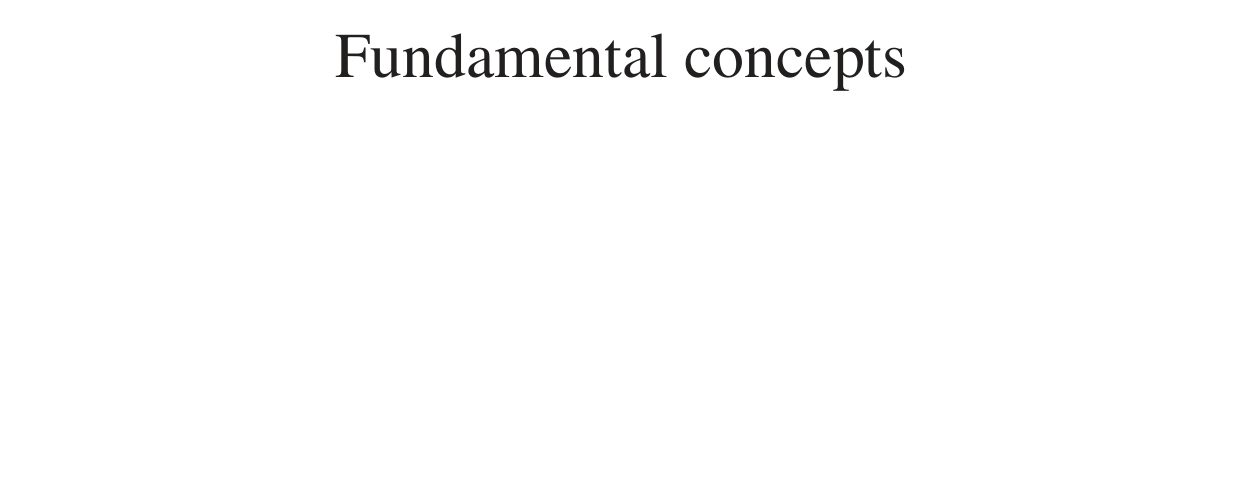
\includegraphics[width=0.55\linewidth]{../Figures/fig_1_1.png}
\caption{图 1.1}
\end{figure}

质点的位置由矢量 $\mathbf{r}$ 确定。

质点的速度定义为它的位置随时间的变化率，质点的加速度定义为它的速度随时间的变化率，即
$$
\mathbf{v} = \frac{d\mathbf{r}}{dt} = \dot{\mathbf{r}}, \eqno\hbox{(1.1)}
$$
和
$$
\mathbf{a} = \frac{d\mathbf{v}}{dt} = \ddot{\mathbf{r}}. \eqno\hbox{(1.2)}
$$
把 $\mathbf{a}$ 表示为 $\mathbf{r}$、$\dot{\mathbf{r}}$ 和 $t$ 的函数的方程，称为运动方程。运动方程是二阶微分方程，其解给出作为时间函数的位置，$\mathbf{r} = \mathbf{r}(t)$。对于任何合理的加速度表达式，运动方程都可以数值求解；对于少数几种加速度表达式，则可以解析求解。你可能会惊讶地听说，求解运动方程的仅有的普适技术，是体现在哈密顿--雅可比方程中的方法，我们将在第 6 章讨论它。你以前接触过的所有解，都是涉及非常简单的加速度的特殊情形。

你在初级物理课程中熟悉的典型问题，涉及落体或抛射体的运动。你会记得，抛射体问题是二维的，因为运动发生在一个平面内。它通常用笛卡尔坐标来描述。

二维运动的另一个重要例子，是质点沿圆或椭圆路径的运动，例如行星绕太阳的轨道运动。由于运动是平面的，物体的位置可以用两个坐标来确定。它们通常是平面极坐标 $(r, \theta)$，其与笛卡尔坐标的关系由下列变换方程给出
$$
x = r\cos\theta,
$$
$$
y = r\sin\theta.
$$
这是一个点变换的例子，其中 $xy$ 平面内的点被映射到 $r\theta$ 平面内的点。

你会记得，在极坐标中，加速度矢量可以分解为一个径向分量和一个方位角分量：
$$
\mathbf{a} = \ddot{\mathbf{r}} = a_r\hat{\mathbf{r}} + a_\theta\hat{\boldsymbol{\theta}}. \eqno\hbox{(1.3)}
$$

\begin{exercise}
给一个质点一个冲量，使其获得速度 $v_0$。随后质点经历加速度 $\mathbf{a} = -b\mathbf{v}$，其中 $b$ 是常数，$\mathbf{v}$ 是速度。求 $v = v(t)$ 和 $x = x(t)$ 的表达式。（这是一维问题。）答案：$x(t) = x_0 + (v_0/b)(1 - e^{-bt})$。
\end{exercise}

\begin{exercise}
假设质量为 $m$ 的物体的加速度由 $a = -(k/m)x$ 给出。（a）写出运动方程。（b）求解运动方程。（c）若物体在 $x = A$ 处由静止释放，确定任意常数（或积分常数）的值。（该运动称为"简谐运动"。）答案（c）：$x = A\sin\left(\sqrt{k/m}\,t + \pi/2\right) = A\cos\left(\sqrt{k/m}\,t\right)$。
\end{exercise}

\begin{exercise}
在平面极坐标中，位置由 $\mathbf{r} = r\hat{\mathbf{r}}$ 给出。用 $r$、$\theta$、$\hat{\mathbf{r}}$、$\hat{\boldsymbol{\theta}}$ 表示速度和加速度。（提示：把 $\hat{\mathbf{r}}$ 和 $\hat{\boldsymbol{\theta}}$ 用 $\hat{\mathbf{i}}$ 和 $\hat{\mathbf{j}}$ 表示。）答案：$\mathbf{a} = (\ddot{r} - r\dot{\theta}^2)\hat{\mathbf{r}} + (r\ddot{\theta} + 2\dot{r}\dot{\theta})\hat{\boldsymbol{\theta}}$。
\end{exercise}

\section*{1.2  广义坐标}

在前一节中，我们说质点的位置由矢量 $\mathbf{r}$ 给出。我们假定了一个惯性笛卡尔坐标系，其中 $\mathbf{r}$ 的分量为 $(x, y, z)$。当然，我们还可以用许多其他方式来确定质点的位置。马上就能想到的方式有：给出矢量 $\mathbf{r}$ 在柱坐标 $(\rho, \phi, z)$ 或球坐标 $(r, \theta, \phi)$ 中的分量。显然，一个具体问题可以用许多不同的坐标组来表述。

在三维空间中，确定单个质点的位置需要三个坐标。对于由两个质点组成的系统，我们需要六个坐标。一个由 $N$ 个质点组成的系统需要 $3N$ 个坐标。在笛卡尔坐标中，两个质点的位置可以用数集 $(x_1, y_1, z_1, x_2, y_2, z_2)$ 来描述。对于 $N$ 个质点，所有质点的位置为
$$
(x_1, y_1, z_1, x_2, y_2, z_2, \ldots, x_N, y_N, z_N).
$$
如你所知，有些问题在一种坐标系中较易求解，而另一些问题在另一种坐标系中较易求解。为避免指明我们所用的坐标系，我们将坐标记作 $q_i$，相应的速度记作 $\dot{q}_i$。我们称 $q_i$ 为"广义坐标"。当然，对于任何具体问题，你都会选取一组合适的坐标；在一个问题中你可能会用球坐标，此时当 $i$ 从 1 到 3 取值时，坐标 $q_i$ 取 $r$、$\theta$、$\phi$；而在另一个问题中，你可能会用柱坐标，此时 $q_i = \rho, \phi, z$。

要从笛卡尔坐标变换到广义坐标，你需要知道变换方程，也就是说，你需要知道下列关系
$$
q_1 = q_1(x_1, y_1, z_1, x_2, y_2, \ldots, z_N, t) \eqno\hbox{(1.4)}
$$
$$
q_2 = q_2(x_1, y_1, z_1, x_2, y_2, \ldots, z_N, t)
$$
$$
\ldots
$$
$$
q_{3N} = q_{3N}(x_1, y_1, z_1, x_2, y_2, \ldots, z_N, t).
$$
逆关系也叫变换方程。对于一个由 $N$ 个质点组成的系统，我们有
$$
x_1 = x_1(q_1, q_2, \ldots, q_{3N}, t) \eqno\hbox{(1.5)}
$$
$$
y_1 = y_1(q_1, q_2, \ldots, q_{3N}, t)
$$
$$
\ldots
$$
$$
z_N = z_N(q_1, q_2, \ldots, q_{3N}, t).
$$
为了方便，常常把所有笛卡尔坐标都用字母 $x$ 表示。于是，对单个质点，$(x, y, z)$ 写成 $(x_1, x_2, x_3)$；对 $N$ 个质点，$(x_1, y_1, \ldots, z_N)$ 表示为 $(x_1, \ldots, x_n)$，其中 $n = 3N$。

我们通常假定，已知由各 $q$ 到各 $x$ 的变换方程，就能进行由各 $x$ 到各 $q$ 的逆变换，但情况并非总是如此。如果方程（1.4）的雅可比行列式不为零，逆变换就是可能的，即
$$
\frac{\partial(q_1, q_2, \ldots, q_n)}{\partial(x_1, x_2, \ldots, x_n)} =
\begin{vmatrix}
\partial q_1/\partial x_1 & \partial q_1/\partial x_2 & \cdots & \partial q_1/\partial x_n\\
\vdots & \vdots & & \vdots\\
\partial q_n/\partial x_1 & \partial q_n/\partial x_2 & \cdots & \partial q_n/\partial x_n
\end{vmatrix} \neq 0.
$$
通常假定广义坐标是线性无关的，因而构成描述问题的极小坐标集。例如，半径为 $a$ 的球面上的质点的位置，可以用两个角（如经度和纬度）来描述。这两个角构成一个由线性无关坐标组成的极小集。然而，我们也可以用三个笛卡尔坐标 $x$、$y$、$z$ 来描述质点的位置。显然，这不是一个极小集。原因是笛卡尔坐标并非全部独立，它们满足关系 $x^2 + y^2 + z^2 = a^2$。注意，给定 $x$ 和 $y$，坐标 $z$ 就确定了。这样的关系称为"约束"。我们发现，每一条约束方程都把独立坐标的数目减少一个。

虽然笛卡尔坐标具有矢量的分量这一性质，但广义坐标未必如此。因此，在我们所说的球面上质点的例子中，两个角是一组合适的广义坐标，但它们并不是矢量的分量。事实上，广义坐标甚至不必是通常意义下的坐标。我们将在后面看到，在某些情形下，广义坐标可以是动量的分量，甚至是没有任何物理解释的量。

当你真正求解问题时，你将使用笛卡尔坐标、柱坐标，或任何对具体问题最方便的坐标系。但在理论工作中，人们几乎总是用广义坐标 $(q_1, \ldots, q_n)$ 来表述问题。你将会看到，广义坐标的概念远不止是一种记法工具。

\begin{exercise}
写出由笛卡尔坐标到球坐标的变换方程。求这个变换的雅可比行列式。说明两个坐标系中的体积元如何与雅可比行列式相联系。答案：$d\tau = r^2\sin\theta\,dr\,d\theta\,d\phi$。
\end{exercise}

\section*{1.3  广义速度}

如前所述，质点在空间中某个特定点的位置，既可以用笛卡尔坐标 $\xi$ 表示，也可以用广义坐标 $q_i$ 表示。它们通过变换方程彼此联系：
$$
\xi = \xi(q_1, q_2, q_3, t).
$$
注意，$\xi$ 是某个特定质点的三个笛卡尔坐标之一，（一般）依赖于所有的广义坐标。

现在我们用广义坐标来确定速度的分量。质点在 $\xi$ 方向上的速度为 $v_i$，按定义
$$
v_i \equiv \frac{d\xi_i}{dt}.
$$
但 $\xi$ 是各 $q$ 的函数，所以利用微分的链式法则，有
$$
v_i = \sum_{k=1}^{n}\frac{\partial \xi}{\partial q_k}\frac{dq_k}{dt} + \frac{\partial \xi}{\partial t} = \sum_{k}\frac{\partial \xi}{\partial q_k}\dot{q}_k + \frac{\partial \xi}{\partial t}. \eqno\hbox{(1.6)}
$$
现在我们来求一个非常有用的关系式，它涉及 $v_i$ 对 $\dot{q}_j$ 的偏导数。由于二阶混合偏导数不依赖于求导的次序，我们可以写出
$$
\frac{\partial}{\partial \dot{q}_j}\frac{\partial \xi}{\partial t} = \frac{\partial}{\partial t}\frac{\partial \xi}{\partial \dot{q}_j}.
$$
但 $\partial\xi/\partial\dot{q}_j = 0$，因为 $x$ 不依赖于广义速度 $\dot{q}$。让我们用方程（1.6）求 $v_i$ 对 $\dot{q}_j$ 的偏导数。这给出
$$
\frac{\partial v_i}{\partial \dot{q}_j} = \frac{\partial}{\partial \dot{q}_j}\sum_{k}\frac{\partial \xi}{\partial q_k}\dot{q}_k + \frac{\partial}{\partial \dot{q}_j}\frac{\partial \xi}{\partial t} = \frac{\partial}{\partial \dot{q}_j}\sum_{k}\frac{\partial \xi}{\partial q_k}\dot{q}_k + 0
$$
$$
= \sum_{k}\frac{\partial}{\partial \dot{q}_j}\left(\frac{\partial \xi}{\partial q_k}\right)\dot{q}_k + \sum_{k}\frac{\partial \xi}{\partial q_k}\frac{\partial \dot{q}_k}{\partial \dot{q}_j} = 0 + \sum_{k}\frac{\partial \xi}{\partial q_k}\delta_{ij} = \frac{\partial \xi}{\partial q_j}.
$$
于是，我们得出结论
$$
\frac{\partial v_i}{\partial \dot{q}_j} = \frac{\partial \xi}{\partial q_j}. \eqno\hbox{(1.7)}
$$
这个简单的关系式在许多涉及广义坐标的推导中非常有用。幸运的是，它很容易记忆，因为它说明：笛卡尔速度与广义速度的关系，与笛卡尔坐标与广义坐标的关系相同。

\section*{1.4  约束}

每个物理系统都有特定数目的自由度。自由度数目是完整确定系统每一部分的位置所需的独立坐标的数目。要描述一个自由质点的位置，必须确定三个坐标（比如 $x$、$y$ 和 $z$）的值。因此，自由质点有三个自由度。对于由两个自由质点组成的系统，你需要确定两个质点的位置。每个质点有三个自由度，所以系统整体有六个自由度。一般说来，由 $N$ 个自由质点组成的力学系统有 $3N$ 个自由度。

当系统受到约束力作用时，往往可以减少描述运动所需的坐标数目。例如，桌子上质点的运动可以用 $x$ 和 $y$ 来描述，约束是 $z$ 坐标（定义为垂直于桌面）由 $z = $ 常数给出。球面上质点的运动可以用两个角来描述，而约束本身可以表示为 $r = $ 常数。每个约束都把自由度的数目减少一个。

在许多问题中，系统以某种方式受到约束。例子有：在桌面表面滚动的弹珠，或沿导线滑动的珠子。在这些问题中，质点不是完全自由的。有某些力作用在它上面，限制它的运动。如果一块冰球在光滑的冰面上滑动，重力向下作用，法向力向上作用。如果冰球离开冰面，法向力就停止作用，重力会很快把它拉回表面。在表面处，法向力阻止冰球继续沿竖直方向向下运动。表面对质点施加的力称为约束力。

如果由 $N$ 个质点组成的系统受到 $k$ 个约束的作用，那么描述运动所需的广义坐标数目为 $3N - k$。（笛卡尔坐标的数目总是 $3N$，但（独立的）广义坐标的数目是 $3N - k$。）

约束是坐标之间的关系。例如，如果一个质点被约束在把抛物线绕 $z$ 轴旋转所形成的抛物面表面上，那么质点的坐标满足关系 $z - x^2/a - y^2/b = 0$。类似地，被约束在球面上的质点，其坐标满足关系 $x^2 + y^2 + z^2 - a^2 = 0$。

如果约束方程（坐标之间的关系）可以表示成
$$
f(q_1, q_2, \ldots, q_n, t) = 0, \eqno\hbox{(1.8)}
$$
的形式，则这个约束称为完整约束。\footnote{不显含时间的约束称为定常约束（scleronomous）。因此，$x^2 + y^2 + z^2 - a^2 = 0$ 既是完整的又是定常的。}

完整约束定义的关键要素是：（1）等号；（2）它是涉及坐标的关系。例如，一个可能的约束是：质点总是处于半径为 $a$ 的球的外部。这个约束可以表示为 $r \geq a$。这不是完整约束。有时约束不仅涉及坐标，还涉及速度或坐标的微分。这样的约束也不是完整的。

作为非完整约束的一个例子，考虑一个在完全粗糙的桌面上滚动的弹珠。弹珠需要五个坐标来完整描述它的位置和取向：两个线坐标给出它在桌面上的位置，三个角坐标描述它的取向。如果桌面是完全光滑的，弹珠可以滑动，线坐标与角坐标之间就没有关系。但是，如果桌面是粗糙的，角坐标与线坐标之间就有关系（约束）。这些约束具有一般形式 $dr = a\,d\theta$，这是微分之间的关系。如果这样的微分表达式可以积分，那么约束就变成坐标之间的关系，它就是完整的。但一般说来，在平面上的滚动并不导致可积分的关系。也就是说，一般而言，滚动约束不是完整的，因为滚动约束是微分之间的关系。约束方程并不仅仅涉及坐标。（但沿直线的滚动是可积的，因而是完整的。）

完整约束是形如（1.8）的、联系广义坐标的方程，它可以用来用一个坐标表示其他坐标，从而减少描述运动所需的坐标数目。

\begin{exercise}
一颗珠子在一根以复杂方式在空间中运动的导线上滑动。这个约束是完整的吗？它是定常的吗？
\end{exercise}

\begin{exercise}
画一幅图，说明弹珠可以在桌面上滚动并回到初始位置但取向不同，而沿直线滚动时角与位置之间存在一一对应关系。
\end{exercise}

\begin{exercise}
写出在椭球面上运动的质点的约束方程。
\end{exercise}

\begin{exercise}
考虑一个双原子分子。假设原子是质点。分子可以转动，也可以沿连接两原子的直线振动。它有几个转动轴？（我们不把终态无法与初态区分的转动计入。）分子有多少个自由度？（答案：6。）
\end{exercise}

\begin{exercise}
在室温下，$\mathrm{O}_2$ 的振动自由度被"冻结"。室温下氧分子有多少个自由度？（答案：5。）
\end{exercise}

\section*{1.5  虚位移}

虚位移 $\delta\xi$ 定义为坐标 $\xi$ 的无穷小瞬时位移，且与作用在系统上的任何约束相容。

为了理解普通位移 $dx_i$ 与虚位移 $\delta\xi$ 之间的差别，考虑变换方程
$$
\xi = \xi(q_1, q_2, \ldots, q_n, t), \qquad i = 1, 2, \ldots, 3N.
$$
对变换方程取微分，我们得到
$$
dx_i = \frac{\partial \xi}{\partial q_1}dq_1 + \frac{\partial \xi}{\partial q_2}dq_2 + \cdots + \frac{\partial \xi}{\partial q_n}dq_n + \frac{\partial \xi}{\partial t}dt = \sum_{\alpha=1}^{n}\frac{\partial \xi}{\partial q_\alpha}dq_\alpha + \frac{\partial \xi}{\partial t}dt.
$$
但对于虚位移 $\delta\xi$，时间是冻结的，所以
$$
\delta\xi = \sum_{\alpha=1}^{n}\frac{\partial \xi}{\partial q_\alpha}\delta q_\alpha. \eqno\hbox{(1.9)}
$$

\section*{1.6  虚功与广义力}

假设一个系统受到若干主动力的作用。设 $F_i$ 是沿 $\xi$ 方向的力分量。（于是，对两质点系统，$F_5$ 将是作用在质点 2 上沿 $y$ 方向的力。）让所有笛卡尔坐标经历虚位移 $\delta\xi$，则主动力所做的虚功为
$$
\delta W = \sum_{i=1}^{3N}F_i\,\delta\xi.
$$
把方程（1.9）中的 $\delta\xi$ 代入，
$$
\delta W = \sum_{i=1}^{3N}F_i\sum_{\alpha=1}^{3N}\frac{\partial \xi}{\partial q_\alpha}\delta q_\alpha.
$$
交换求和次序，
$$
\delta W = \sum_{\alpha=1}^{3N}\left(\sum_{i=1}^{3N}F_i\frac{\partial \xi}{\partial q_\alpha}\right)\delta q_\alpha.
$$
回想"功等于力乘以距离"这一基本概念，我们定义广义力为
$$
Q_\alpha = \sum_{i=1}^{3N}F_i\frac{\partial \xi}{\partial q_\alpha}. \eqno\hbox{(1.10)}
$$
于是虚功可以表示为
$$
\delta W = \sum_{\alpha=1}^{3N}Q_\alpha\,\delta q_\alpha.
$$
方程（1.10）就是广义力的定义。

\begin{example}
证明虚功原理（平衡时 $\delta W = 0$）蕴含着作用在物体上的力矩之和必须为零。

\textbf{解 1.1：}选一个沿任意方向的转轴。设物体绕该轴转过一个无穷小角度 $\epsilon$。位于 $\mathbf{R}_i$ 处的点 $P_i$ 相对于轴的虚位移由下式给出
$$
\delta\mathbf{R}_i = \boldsymbol{\epsilon}\times\mathbf{R}_i.
$$
作用在 $P_i$ 上的力 $\mathbf{F}_i$ 所做的功为
$$
\delta W_i = \mathbf{F}_i\cdot\delta\mathbf{R}_i = \mathbf{F}_i\cdot(\boldsymbol{\epsilon}\times\mathbf{R}_i) = \boldsymbol{\epsilon}\cdot(\mathbf{R}_i\times\mathbf{F}_i) = \boldsymbol{\epsilon}\cdot\mathbf{N}_i,
$$
其中 $\mathbf{N}_i$ 是绕轴作用在 $P_i$ 上的力矩。总的虚功为
$$
\delta W = \sum_i \boldsymbol{\epsilon}\cdot\mathbf{N}_i = \boldsymbol{\epsilon}\cdot\sum_i\mathbf{N}_i = \boldsymbol{\epsilon}\cdot\mathbf{N}_{\mathrm{tot}}.
$$
对不转动的物体，$\boldsymbol{\epsilon}$ 的方向是任意的，所以 $\mathbf{N}_{\mathrm{tot}} = 0$。
\end{example}

\begin{exercise}
考虑一个由笛卡尔坐标描述的、由四个质点组成的系统。$F_{10}$ 是什么？
\end{exercise}

\begin{exercise}
一个质点受到分量为 $F_x$ 和 $F_y$ 的力作用。求极坐标中的广义力。答案：$Q_r = F_x\cos\theta + F_y\sin\theta$，$Q_\theta = -F_xr\sin\theta + F_yr\cos\theta$。
\end{exercise}

\begin{figure}[h]
\centering
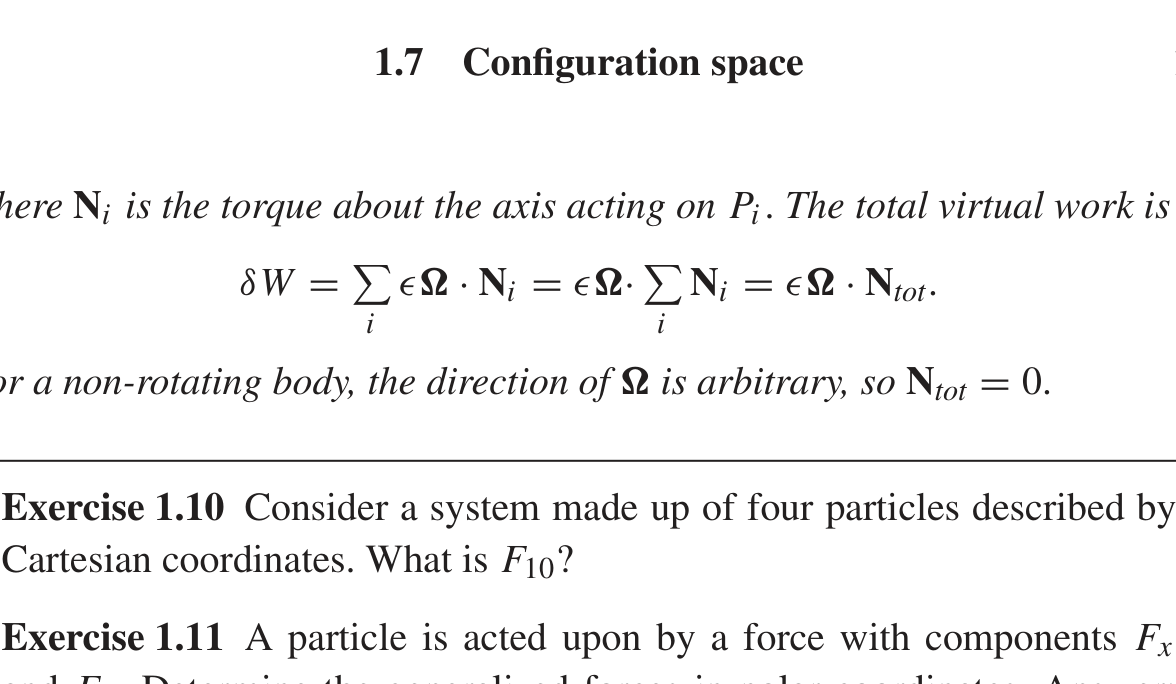
\includegraphics[width=0.55\linewidth]{../Figures/fig_1_2.png}
\caption{图 1.2}
\end{figure}

两个处于平衡的物块。

\begin{exercise}
利用虚功证明：平衡要求 $M = m/\sin\theta$。（这用初等方法即可容易地证明，但要求你用虚功来解这道题。）
\end{exercise}

\section*{1.7  位形空间}

确定系统中所有质点的位置，称为系统的位形。一般说来，由 $N$ 个自由质点组成的系统的位形由下式给出
$$
(q_1, q_2, \ldots, q_n), \quad \text{其中 } n = 3N. \eqno\hbox{(1.11)}
$$
考虑单个质点。它在笛卡尔坐标中的位置由 $x$、$y$、$z$ 给出，在直线三维参考系中，质点的位置用一个点表示。对于由两个质点组成的系统，你可以用两个点来表示系统的位形。然而，（至少在概念上）你也可以用六维参考系中的一个点来表示位形。在这个六维空间中，有六个相互垂直的轴，分别标为 $x_1, y_1, z_1, x_2, y_2, z_2$。类似地，由 $N$ 个质点组成的系统的位形，用 $3N$ 维参考系中的一个点表示。

这样一个多维参考系的轴不一定是笛卡尔轴。各个质点的位置可以用球坐标、柱坐标或广义坐标 $q_1, q_2, \ldots, q_n$ 表示。于是，由两个质点组成的系统的位形表示为 $(q_1, q_2, \ldots, q_6)$，其中在笛卡尔坐标中 $q_1 = x_1$，$q_2 = y_1$，$\ldots$，$q_6 = z_2$。在球坐标中，$q_1 = r_1$，$q_2 = \theta_1$，$\ldots$，$q_6 = \phi_2$，对其他任何坐标系也类似。

考虑单个质点的三维参考系。随着时间推移，坐标的值发生变化。这种变化是连续的，表示质点位置的点将描绘出一条光滑曲线。类似地，在以广义坐标为轴、维数为 $n$ 的位形空间中，表示系统位形的点将描绘出一条光滑曲线，它表示系统的时间演化。
\begin{figure}[h]
\centering
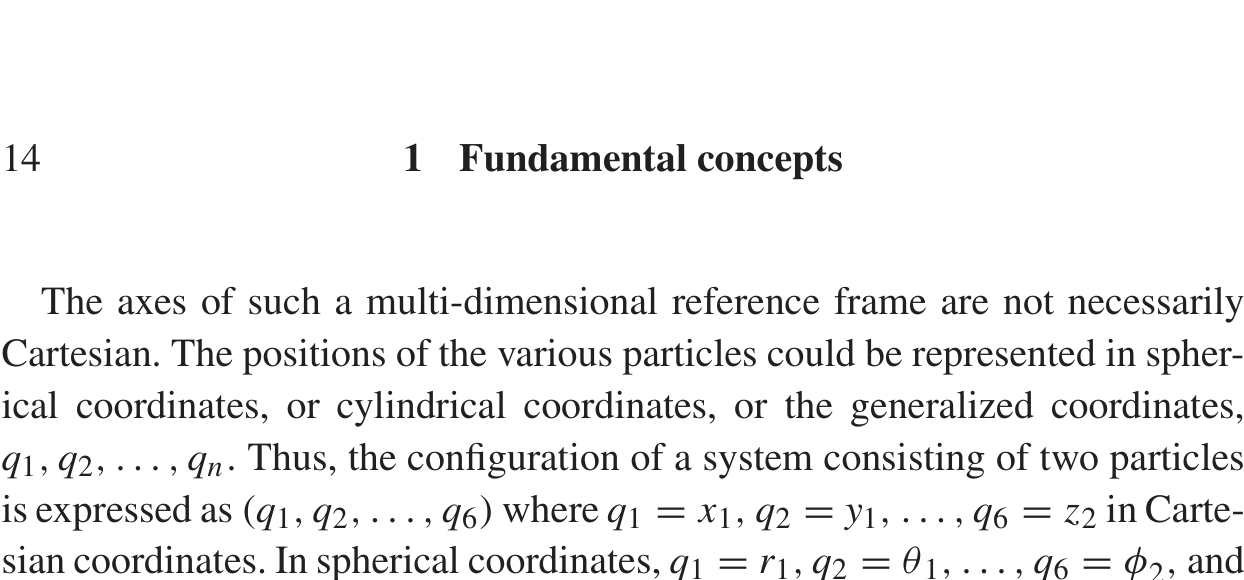
\includegraphics[width=0.55\linewidth]{../Figures/fig_1_3.png}
\caption{图 1.3}
\end{figure}

位形空间中的一条路径。注意，时间是给出位形点沿曲线位置的参数。

也许值得指出，当我们从一组坐标变换到另一组坐标时，位形空间的特征可能发生显著变化。直线可能变成曲线，角和距离可能改变。然而，某些几何性质保持不变。点仍然是点，曲线仍然是曲线。相邻的曲线保持相邻，一个点的邻域保持为该点的邻域（虽然邻域的形状可能会不同）。

\begin{exercise}
一个质点沿 $r$ 为常数的直线从 $\theta_1$ 运动到 $\theta_2$。证明这在 $r$--$\theta$ 空间中是一条直线，但在 $x$--$y$ 空间中不是直线。
\end{exercise}

\begin{exercise}
方程 $y = 3x + 2$ 在二维笛卡尔空间中描述一条直线。确定这条曲线在 $r$--$\theta$ 空间中的形状。
\end{exercise}

\section*{1.8  相空间}

用质点的位置和动量来描述质点系统往往很方便。系统的"状态"用某一时刻所有质点的位置和动量的值来描述。例如，我们可以用笛卡尔坐标 $\xi$、$i = 1, 2, 3$ 来表示质点的位置。类似地，质点的动量可以用 $p_i$、$i = 1, 2, 3$ 表示。想象画一个 $2n$ 维坐标系，其轴标为 $x_1, \ldots, x_n$；$p_1, \ldots, p_n$。由这组轴所描述的空间称为相空间。所有质点的位置以及所有质点的动量，由相空间中的单个点来表示。随着时间推进，每个质点的位置和动量都发生变化。这些变化是连续的，所以相空间中的点在 $2n$ 维坐标系中连续运动。也就是说，系统的时间演化可以用相空间中的一条轨迹来表示。这条轨迹称为"相路径"，在某些文献中也称为"世界线"。\footnote{相空间的概念在混沌系统的研究中非常重要，在那里，通过分析系统轨迹与相空间中某个特定平面的交集（即所谓的"截面"），可以确定是否正在发生混沌运动。此外，在统计力学中，刘维尔的一个基本定理表明：如果画出系统系综的相空间轨迹，那么在给定系统附近的相空间点的密度将随时间保持不变。}

我们很快就会定义"广义动量"，然后相空间将用广义坐标 $(q_1, \ldots, q_n)$ 和广义动量 $(p_1, \ldots, p_n)$ 来描述。

\section*{1.9  动力学}

\subsection*{1.9.1  牛顿运动定律}

动力学是研究决定物体运动规律的学科。你第一次接触动力学，几乎肯定是从学习艾萨克·牛顿的三大定律开始的。

（1）第一定律，即惯性定律：不受任何外力作用的物体，将以恒定速度沿直线运动。

（2）第二定律，即运动方程：物体动量的变化率等于作用在它上面的合外力。

（3）第三定律，即作用与反作用：若一物体对第二个物体施加一个力，则第二个物体对第一个物体施加一个大小相等、方向相反、性质相同的力。

第一定律告诉我们，自由质点将以恒定速度运动。

第二定律通常用矢量关系表示
$$
\mathbf{F} = \frac{d\mathbf{p}}{dt}. \eqno\hbox{(1.12)}
$$
如果质量恒定，这个关系就化为众所周知的方程
$$
\mathbf{F} = m\mathbf{a}.
$$
第三定律可以表示为强形式，也可以表示为弱形式。强形式说明力大小相等、方向相反，且沿连接两质点的直线方向作用。第三定律的弱形式只说明力大小相等、方向相反。

这些定律（尤其是第二定律）在解决实际问题时极其有用。

\subsection*{1.9.2  运动方程}

第二定律常常用来确定受到各种不平衡力作用的物体的加速度。用位置和速度表示加速度的方程称为"运动方程"。（在初级物理课程中，求加速度涉及隔离系统、画受力图，然后应用第二定律，通常用 $F = ma$ 的形式。）由于力可以用位置、速度和时间表示，第二定律给出的加速度表达式具有如下形式
$$
\ddot{x} = \ddot{x}(x, \dot{x}, t).
$$
这就是运动方程。然后，通过对运动方程积分两次，可以确定质点作为时间函数的位置，
$$
x = x(t).
$$
这个过程称为确定运动。

牛顿定律简单而直观，是大多数初等力学课程的基础。偶尔引用它们是方便的，但我们的研究并非以牛顿定律为基础。

\subsection*{1.9.3  牛顿与莱布尼茨}

众所周知，艾萨克·牛顿和戈特弗里德·莱布尼茨各自独立地发明了微积分。不太为人所知的是，他们对质点系统的时间演化有不同的看法。牛顿第二定律给出了作用在质点上的力与其加速度之间的矢量关系。（对于由 $N$ 个质点组成的系统，我们有 $N$ 个矢量关系，对应 $3N$ 个标量二阶微分方程。这些方程通常是耦合的，因为所有 $N$ 个质点的位置都可能出现在 $3N$ 个运动方程中的每一个里面。要确定运动，我们必须同时求解所有这些耦合方程。）

另一方面，莱布尼茨认为，通过考察质点的"活力"（vis viva），或者用我们今天的话说，它们的动能，可以更好地分析质点的运动。

从根本上说，牛顿认为量 $m_iv_i$ 在运动过程中是守恒的，而莱布尼茨认为 $m_iv_i^2$ 是常数。用现代术语来说，牛顿相信动量守恒，而莱布尼茨相信动能守恒。不久就清楚了，动能（$T$）在系统运动过程中并不守恒，但当势能（$V$）的概念引入后，莱布尼茨的理论被扩展为：总能量（$E = T + V$）是常数，这当然是力学的基本守恒定律之一。因此，你可以说，牛顿和莱布尼茨都是正确的。

在初级物理课程中，你经常在牛顿定律和能量守恒之间切换使用。例如，落体问题可以用 $F = ma$ 求解，也可以用能量守恒求解。

后来，欧拉和拉格朗日发展了莱布尼茨的思想，并表明系统的运动可以由一个统一的原理来预言，我们现在称之为哈密顿原理。有意思的是，这种方法不涉及矢量，甚至不涉及力，尽管力可以从它导出。欧拉和拉格朗日的方法称为"分析力学"，它是我
们研究的主要焦点。（由于牛顿的方法为你所非常熟悉，我们在考虑物理问题的某些方面时，会偶尔使用它。）

分析力学不要求牛顿三大定律，尤其不需要第三定律。有些物理学家认为，牛顿引入第三定律是为了处理约束问题。（弹跳的球被"约束"在房间内。在牛顿的图像中，球从墙上弹回，是因为墙对它施加了一个反作用力，正如第三定律所给出的那样。）拉格朗日方法把约束纳入分析的框架，第二定律和第三定律都不是必需的。然而，约束力和运动方程都可以由该方法确定。此外，分析力学中的所有方程都是标量方程，所以我们不需要使用矢量分析的任何概念。不过，有时矢量很方便，我们会偶尔使用它们。

本书致力于用变分原理发展分析力学的概念和技术。\footnote{请注意，分析力学和变分法领域非常广阔，本书只限于介绍一些基本概念。}我相信你会发现这是一套非常优美、非常有力的理论。在一本这方面的知名著作的引言中，作者谈到自己时说："他一次又一次地体验到那种由于专注于分析力学的基本原理和方法而伴随而来的异乎寻常的心灵狂喜。"（你可能不会感到"心灵的狂喜"，但我认为你会领会这位作者所表达的意思。）\footnote{Cornelius Lanczos，《力学的变分原理》(The Variational Principles of Mechanics)，多伦多大学出版社，1970 年。纽约多佛出版社（Dover Press）1986 年再版。}

\section*{1.10  求运动方程}

在本节中，我们回顾求解运动方程的方法。正如你可能预料的那样，求解运动方程会得到运动的一个表达式，即位置作为时间的函数。碰巧，表达运动方程有好几种不同的方式，但此刻让我们把它看作是质点加速度的表达式，用系统中其他所有质点的位置和速度来表示。

正如朗道和栗弗席兹所指出的，\footnote{L. D. Landau and E. M. Lifshitz，Mechanics，A Course of Theoretical Physics 第 1 卷，Pergamon Press，Oxford，1976，p.1。}"如果所有坐标和速度同时确定，那么根据经验，系统的状态就完全确定了，其后续运动原则上可以计算出来。在数学上，这意味着如果在某一时刻给出了所有的坐标 $q$ 和速度 $\dot{q}$，那么该时刻的加速度 $\ddot{q}$ 就唯一确定了。"

换句话说，运动方程可以表示为如下类型的关系：
$$
\ddot{q}_i = \ddot{q}_i(q_1, q_2, \ldots, q_n; \dot{q}_1, \dot{q}_2, \ldots, \dot{q}_n; t).
$$
如果我们知道质点的加速度（$\ddot{q}_i$），那么我们（原则上）就能确定随后某一时刻的位置和速度。因此，知道了运动方程，我们就能预言系统的时间演化。

\subsection*{1.10.1  牛顿力学中的运动方程}

如果质量恒定，求运动方程的一种初等方法是使用如下形式的牛顿第二定律
$$
\ddot{\mathbf{r}} = \mathbf{F}/m. \eqno\hbox{(1.13)}
$$
这是关于 $\mathbf{r}$ 的二阶微分方程，原则上可以求解而得到 $\mathbf{r} = \mathbf{r}(t)$。当然，这需要有 $\mathbf{F}$ 作为 $\mathbf{r}$、$\dot{\mathbf{r}}$ 和 $t$ 的函数的表达式。

作为一个简单的一维例子，考虑一个连接到劲度系数为 $k$ 的弹簧上的质量 $m$。弹簧作用在质量上的力为 $F = -kx$。因此，牛顿第二定律给出如下运动方程
$$
m\ddot{x} + kx = 0. \eqno\hbox{(1.14)}
$$
重要的是要注意，第二定律只适用于惯性坐标系。牛顿意识到了这个问题，他说第二定律是一个在相对于固定恒星静止的坐标系中成立的关系。

\subsection*{1.10.2  拉格朗日力学中的运动方程}

求运动方程的另一种方法是使用拉格朗日技术。当处理质点或可以当作质点处理的刚体时，拉格朗日量可以定义为动能与势能之差。\footnote{虽然方程（1.15）对质点系统完全正确，但在第 7 章考虑连续系统时，我们将得到一个稍微不同的表达式。一般说来，拉格朗日量被定义为一个生成运动方程的函数。}即
$$
L = T - V. \eqno\hbox{(1.15)}
$$
例如，如果质量 $m$ 连接到劲度系数为 $k$ 的弹簧上，势能为 $V = \frac{1}{2}kx^2$，动能为 $T = \frac{1}{2}mv^2 = \frac{1}{2}m\dot{x}^2$。因此拉格朗日量为
$$
L = T - V = \frac{1}{2}m\dot{x}^2 - \frac{1}{2}kx^2.
$$
通常很容易在所采用的任何坐标集中写出势能，但动能的表达式可能有些难以确定，所以只要可能，就应该从笛卡尔坐标出发。在笛卡尔坐标系中，动能具有特别简单的形式，即速度平方的和。即
$$
T = \frac{1}{2}m(\dot{x}^2 + \dot{y}^2 + \dot{z}^2).
$$
要用其他坐标系表示动能，就需要一组变换方程。

例如，对长度为 $l$ 的单摆，势能为 $V = -mgl\cos\theta$，动能为 $T = \frac{1}{2}mv^2 = \frac{1}{2}m(l\dot{\theta})^2$。（这里 $\theta$ 是绳与垂线之间的夹角。）因此拉格朗日量为
$$
L = T - V = \frac{1}{2}ml^2\dot{\theta}^2 + mgl\cos\theta.
$$
动能是速度的函数。（你熟悉诸如 $T = \frac{1}{2}m\dot{x}^2$ 和 $T = \frac{1}{2}ml^2\dot{\theta}^2$ 的表达式。）速度是位置坐标对时间的导数（$\dot{x}$ 和 $l\dot{\theta}$）。势能通常只是位置的函数。在广义坐标中，位置表示为 $q$，速度表示为 $\dot{q}$。因此，拉格朗日量是 $q$ 和 $\dot{q}$ 的函数。即 $L = L(q, \dot{q})$，或更一般地，$L = L(q, \dot{q}, t)$。如果我们关心的是可在三维空间中自由运动的单个质点，那么就有三个 $q$ 和三个 $\dot{q}$。于是 $L = L(q_1, q_2, q_3, \dot{q}_1, \dot{q}_2, \dot{q}_3, t)$。对由 $N$ 个质点组成的系统，若 $n = 3N$，我们写
$$
L = L(q_i, \dot{q}_i, t), \qquad i = 1, \ldots, n.
$$
我假定你在中级力学课程中已经接触过拉格朗日量和拉格朗日方程。在接下来的两章中，你会看到从第一原理出发对拉格朗日方程的推导。不过，此刻我直接写出该方程而不加证明，并向你展示如何把它作为求运动方程的工具来使用。

对单个坐标 $q$，拉格朗日方程为
$$
\frac{d}{dt}\frac{\partial L}{\partial \dot{q}} - \frac{\partial L}{\partial q} = 0. \eqno\hbox{(1.16)}
$$
如果有 $n$ 个坐标，就有 $n$ 个拉格朗日方程，即
$$
\frac{d}{dt}\frac{\partial L}{\partial \dot{q}_i} - \frac{\partial L}{\partial q_i} = 0, \qquad i = 1, \ldots, n. \eqno\hbox{(1.17)}
$$
重要的是要认识到，拉格朗日方程就是系统的运动方程。

例如，对弹簧上的质量，拉格朗日量为 $L = T - V = \frac{1}{2}m\dot{x}^2 - \frac{1}{2}kx^2$。把它代入拉格朗日方程，我们得到
$$
\frac{d}{dt}\frac{\partial L}{\partial \dot{x}} - \frac{\partial L}{\partial x} = 0,
$$
$$
\frac{d}{dt}\frac{\partial}{\partial \dot{x}}\left(\frac{1}{2}m\dot{x}^2 - \frac{1}{2}kx^2\right) - \frac{\partial}{\partial x}\left(\frac{1}{2}m\dot{x}^2 - \frac{1}{2}kx^2\right) = 0,
$$
$$
\frac{d}{dt}(m\dot{x}) - kx = 0,
$$
所以
$$
m\ddot{x} + kx = 0,
$$
正如所料。（与方程（1.14）比较。）

为了说明用拉格朗日方程求运动方程的用法，我们考虑几个简单的力学系统。
\begin{figure}[h]
\centering
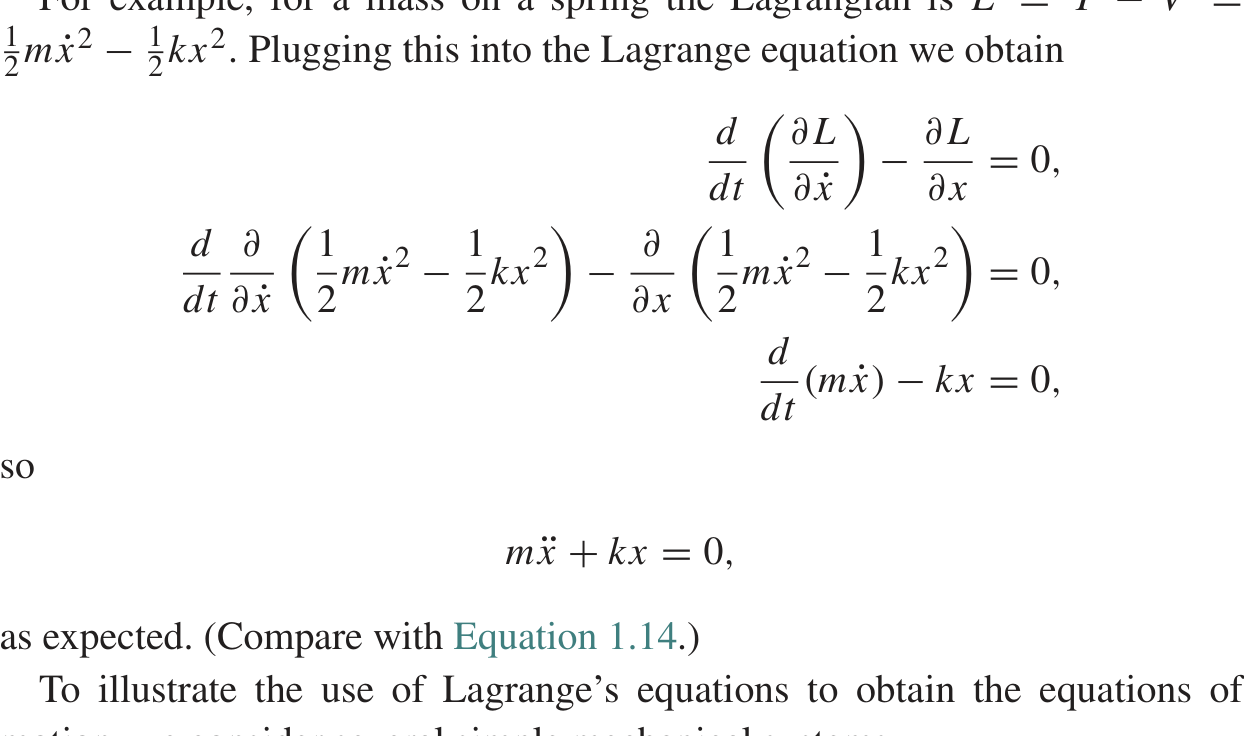
\includegraphics[width=0.55\linewidth]{../Figures/fig_1_4.png}
\caption{图 1.4}
\end{figure}

阿特伍德机。

\begin{example}
考虑一台阿特伍德机。它由质量 $m_1$ 和 $m_2$ 组成，二者由一根无质量的不可伸长的绳子悬挂，绳子跨过一只无摩擦、无质量的滑轮。求拉格朗日量并写出运动方程。

\textbf{解 1.2：}质量的动能为
$$
T = \frac{1}{2}m_1\dot{x}_1^2 + \frac{1}{2}m_2\dot{x}_2^2,
$$
势能为
$$
V = -m_1gx_1 - m_2gx_2,
$$
其中我们选取滑轮中心处 $V = 0$。系统受到约束 $x_1 + x_2 = l = $ 常数。拉格朗日量为
$$
L = T - V = \frac{1}{2}m_1\dot{x}_1^2 + \frac{1}{2}m_2\dot{x}_2^2 + m_1gx_1 + m_2gx_2.
$$
但利用 $x_2 = l - x_1$，我们可以把拉格朗日量用单个变量重新写出，
$$
L = \frac{1}{2}m_1\dot{x}_1^2 + \frac{1}{2}m_2\dot{x}_1^2 + m_1gx_1 + m_2g(l - x_1) = \frac{1}{2}(m_1 + m_2)\dot{x}_1^2 + (m_1 - m_2)gx_1 + m_2gl.
$$
运动方程为
$$
\frac{d}{dt}\frac{\partial L}{\partial \dot{x}_1} - \frac{\partial L}{\partial x_1} = 0,
$$
$$
\frac{d}{dt}(m_1 + m_2)\dot{x}_1 - (m_1 - m_2)g = 0,
$$
$$
\ddot{x}_1 = \frac{m_1 - m_2}{m_1 + m_2}g.
$$
\end{example}

\begin{example}
半径为 $a$、质量为 $m$ 的圆柱体在半径为 $b$ 的固定圆柱体上无滑动地滚动。求拉格朗日量并写出运动方程。

\textbf{解 1.3：}较小圆柱体的动能，是其质心的平动动能加上绕质心转动的动能。即
$$
T = \frac{1}{2}m\left(\dot{r}^2 + r^2\dot{\theta}^2\right) + \frac{1}{2}I\dot{\phi}^2,
$$
其中 $r$ 是两个圆柱体中心之间的距离，$I = \frac{1}{2}ma^2$。势能为 $V = mgr\cos\theta$。因此
$$
L = \frac{1}{2}m(\dot{r}^2 + r^2\dot{\theta}^2) + \frac{1}{2}I\dot{\phi}^2 - mgr\cos\theta.
$$
但有两个约束，即 $r = a + b$ 和 $a\phi = b\theta$。因此 $\dot{r} = 0$，$\dot{\phi} = (b/a)\dot{\theta}$。于是
$$
L = \frac{1}{2}m(a + b)^2\dot{\theta}^2 + \frac{1}{2}ma^2\left(\frac{b}{a}\dot{\theta}\right)^2 - mg(a + b)\cos\theta = \frac{1}{2}m\left(a^2 + 2ab + \frac{3}{2}b^2\right)\dot{\theta}^2 - mg(a + b)\cos\theta,
$$
运动方程为
$$
\frac{d}{dt}\frac{\partial L}{\partial \dot{q}} - \frac{\partial L}{\partial q} = 0
$$
或
$$
m\left(a^2 + 2ab + \frac{3}{2}b^2\right)\ddot{\theta} - mg(a + b)\sin\theta = 0.
$$
\end{example}
\begin{figure}[h]
\centering
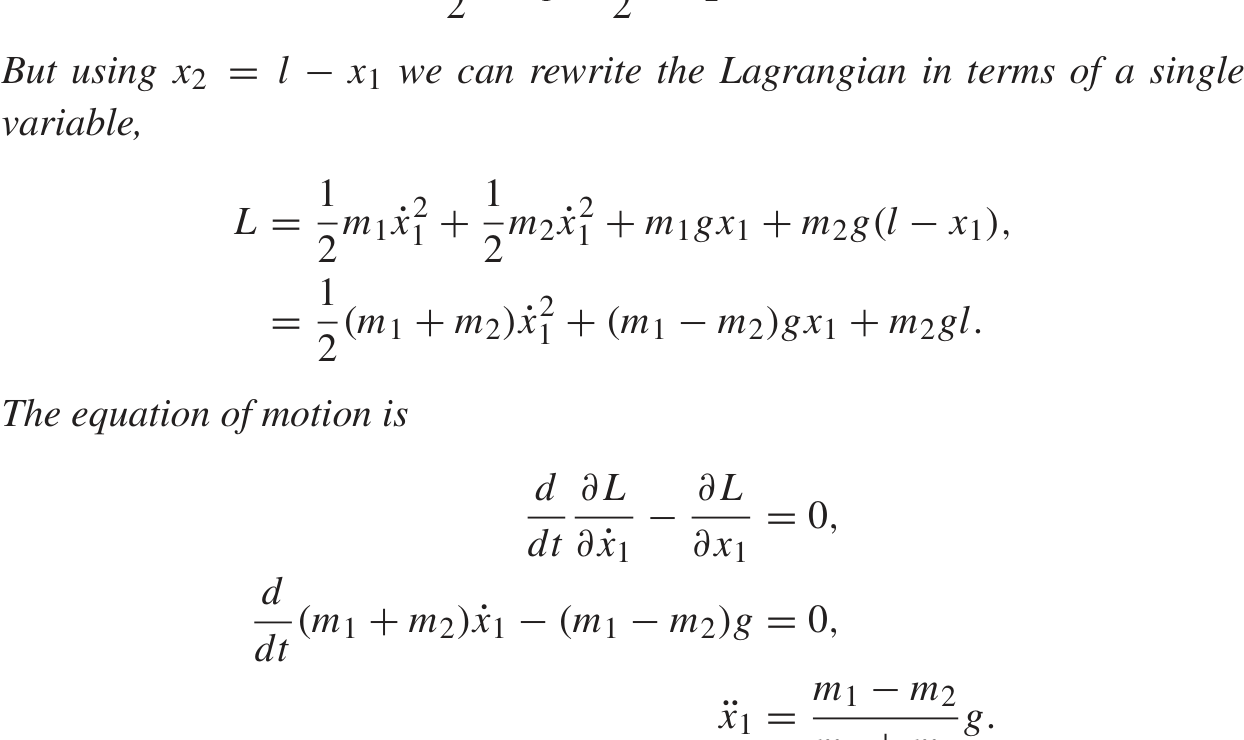
\includegraphics[width=0.55\linewidth]{../Figures/fig_1_5.png}
\caption{图 1.5}
\end{figure}

一个圆柱在另一个圆柱上滚动。

\begin{example}
质量为 $m$ 的小珠在半径为 $a$ 的大质量无摩擦圆环上滑动。圆环绕竖直轴以恒定的角速度 $\omega$ 转动。见图 1.6。

\textbf{解 1.4：}如果圆环质量足够大，小珠的运动不会影响圆环的转速。因此我们忽略圆环的能量。动能是小珠因圆环转动而具有的能量，加上小珠因在圆环上运动（与角度 $\theta$ 的变化有关）而具有的动能。因此
$$
L = \frac{1}{2}ma^2\dot{\theta}^2 + \frac{1}{2}ma^2\omega^2\sin^2\theta + mga\cos\theta.
$$
运动方程为
$$
ma^2\ddot{\theta} - ma^2\omega^2\sin\theta\cos\theta + mga\sin\theta = 0.
$$
\end{example}
\begin{figure}[h]
\centering
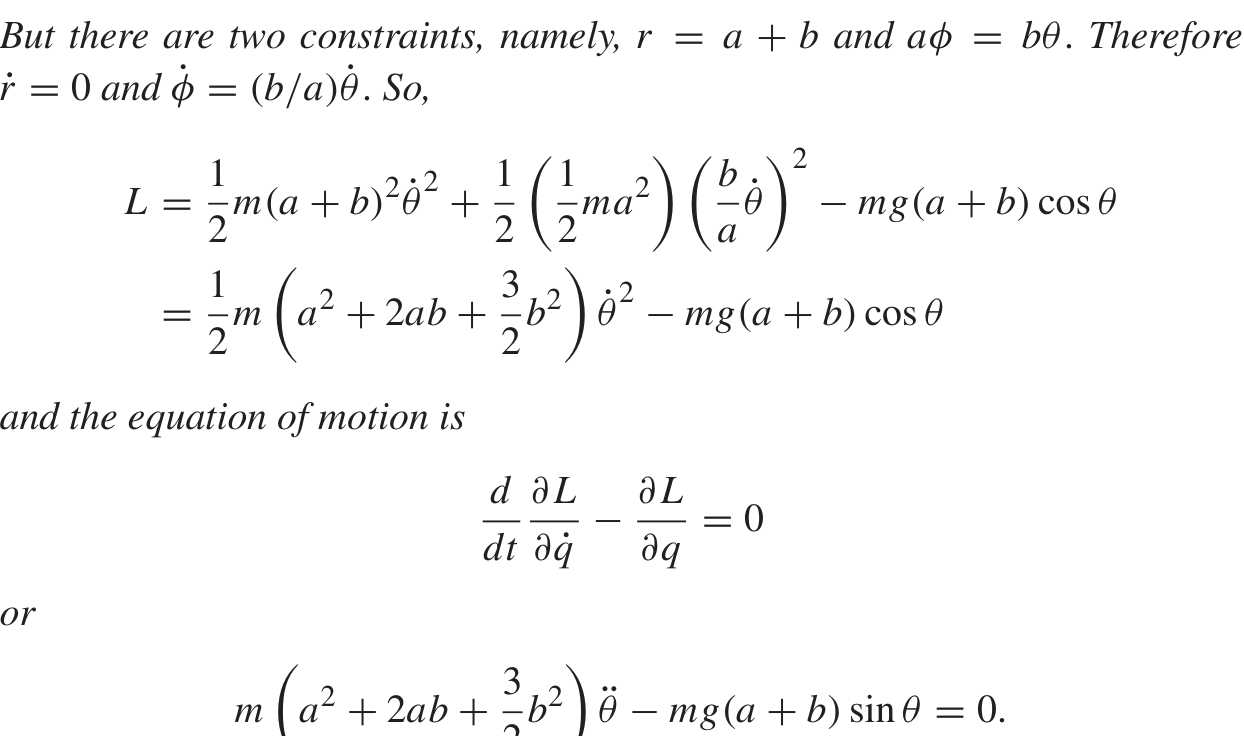
\includegraphics[width=0.55\linewidth]{../Figures/fig_1_6.png}
\caption{图 1.6}
\end{figure}

小珠在转动的圆环上滑动。

\begin{example}
球面摆由一个质量为 $m$ 的摆锤和一根长度为 $l$ 的不可伸长绳子组成。求拉格朗日量并写出运动方程，其中 $\theta$ 是自正 $z$ 轴量起的极角，$\phi$ 是在 $x$--$y$ 平面内自 $x$ 轴量起的方位角。

\textbf{解 1.5：}拉格朗日量为
$$
L = \frac{1}{2}m(\dot{x}^2 + \dot{y}^2 + \dot{z}^2) - mgz.
$$
但
$$
x = l\sin\theta\cos\phi, \qquad y = l\sin\theta\sin\phi, \qquad z = l\cos\theta,
$$
所以
$$
L = \frac{1}{2}ml^2(\dot{\theta}^2 + \sin^2\theta\,\dot{\phi}^2) - mgl\cos\theta.
$$
运动方程为
$$
\frac{d}{dt}(ml^2\dot{\theta}) - ml^2\dot{\phi}^2\sin\theta\cos\theta - mgl\sin\theta = 0,
$$
$$
\frac{d}{dt}(ml^2\sin^2\theta\,\dot{\phi}) = 0.
$$
\end{example}
\begin{figure}[h]
\centering
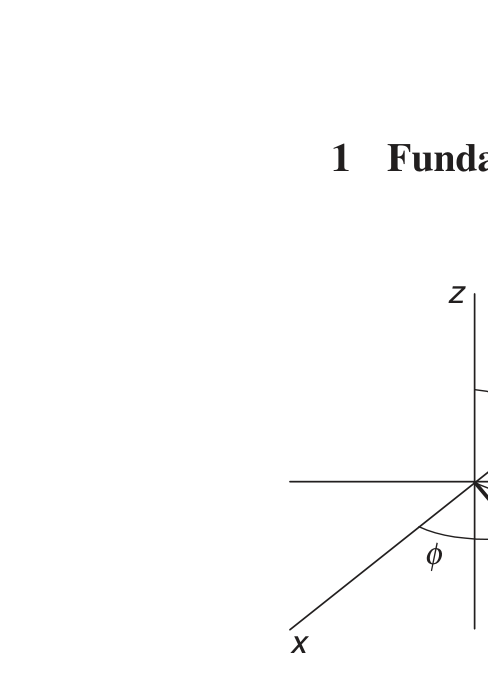
\includegraphics[width=0.55\linewidth]{../Figures/fig_1_7.png}
\caption{图 1.7}
\end{figure}

球面摆。

\begin{exercise}
如果滑轮的转动惯量为 $I$，求阿特伍德机的拉格朗日量和运动方程。答案：$a = g(m_2 - m_1)/(m_1 + m_2 + I/R^2)$。
\end{exercise}

\begin{exercise}
求单摆和双平面摆的拉格朗日量。（假设运动是平面的。）答案：对双摆，
$$
L = \frac{1}{2}(m_1 + m_2)l_1^2\dot{\theta}_1^2 + \frac{1}{2}m_2\left(l_2^2\dot{\theta}_2^2 + 2l_1l_2\dot{\theta}_1\dot{\theta}_2\cos(\theta_1 - \theta_2)\right) + m_1gl_1\cos\theta_1 + m_2g(l_1\cos\theta_1 + l_2\cos\theta_2).
$$
\end{exercise}
\begin{figure}[h]
\centering
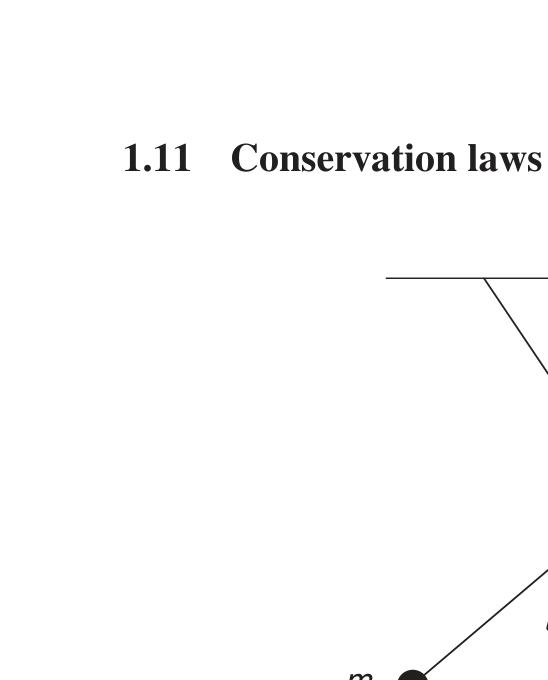
\includegraphics[width=0.55\linewidth]{../Figures/fig_1_8.png}
\caption{图 1.8}
\end{figure}

双平面摆。

\begin{exercise}
飞球调速器是控制电机转速的简单机械装置。当装置越转越快时，质量 $m_2$ 上升。角 $\theta$ 由一根杆与中心轴构成，角 $\phi$ 是绕轴的转动角。任一时刻的角速度为 $\omega = \dot{\phi}$。假设系统处于均匀引力场中。证明拉格朗日量由下式给出
$$
L = m_1a^2(\dot{\theta}^2 + \omega^2\sin^2\theta) + 2m_2a^2\dot{\theta}^2\sin^2\theta + 2(m_1 + m_2)ga\cos\theta.
$$
\end{exercise}
\begin{figure}[h]
\centering
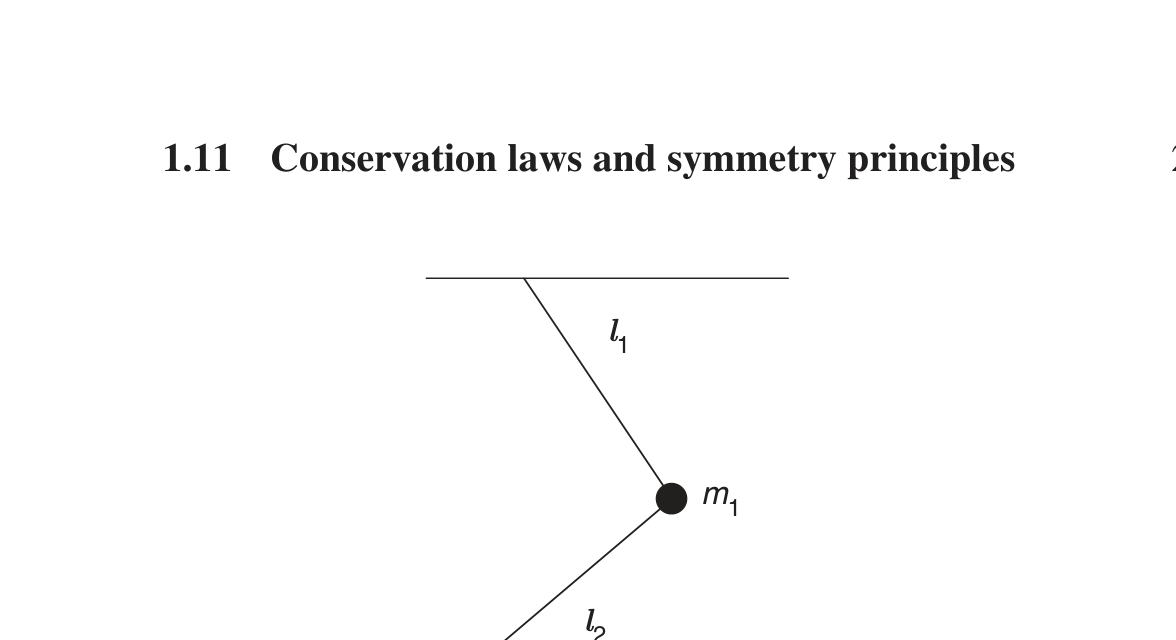
\includegraphics[width=0.55\linewidth]{../Figures/fig_1_9.png}
\caption{图 1.9}
\end{figure}

飞球调速器。

\section*{1.11  守恒定律与对称性原理}

经典力学中三个最重要的守恒定律是：线性动量守恒、角动量守恒和能量守恒。虽然你对这些定律非常熟悉，但用广义坐标和拉格朗日量来考察它们很有意思。我们将证明，这三个基本守恒定律是空间均匀性、空间各向同性和时间均匀性的结果。

当我们说空间的一个区域是均匀的，我们的意思是，它在某个位置与在另一个位置完全相同。因此，系统不会因从一个点位移到另一个点而受影响。举个简单的例子，我断言我的落地大摆钟在房间的一侧和在另一侧的行为相同（但它在月球上的行为就会不同）。

类似地，如果空间是各向同性的，那么它在所有方向上都相同，物理系统在转动下保持不变。我的落地大摆钟在我把它绕竖直轴转过 $90^\circ$ 之后行为相同。但是，我房间里的空间对绕水平轴的转动不是各向同性的。（当我把落地大摆钟倒置时，它就停止了工作。）

最后，如果时间是均匀的，物理系统在两个不同的时刻行为相同。我的时钟今天的行为与上周相同。时间在另一种意义上也是各向同性的，即无论时间正向还是反向流逝，物理系统的行为都相同。

当我们说一个系统具有某种对称性时，我们的意思是，系统对某个特定坐标的改变是不变的。例如，球是一个无论怎样转动看起来都相同的物体。球对称性蕴含着对转动的不变性，即对物体角取向的改变的不变性。类似地，如果系统在沿某个特定方向位移后保持不变，我们就说它在该方向具有平移对称性。当系统对时间的改变保持不变时，我们说它具有时间对称性。

作为平移对称性的一个例子，考虑在均匀竖直引力场中、处于无限水平面上的一个物体。如果物体在水平面内移动，系统保持不变。但是，如果物体竖直移动（如果它被抬高），势能就会改变。因此，这个系统在水平面内具有平移对称性，但对竖直位移不具有平移对称性。在没有力作用的区域，空间在所有三个方向都是均匀的。

一个力学系统完全由其拉格朗日量来描述。如果拉格朗日量不显含某个特定坐标 $q_i$，那么 $q_i$ 的改变不会影响系统。我们就说该系统对 $q_i$ 的改变是对称的。

\subsection*{1.11.1  广义动量与循环坐标}

\subsubsection*{广义动量}

自由质点由拉格朗日量描述
$$
L = \frac{1}{2}m(\dot{x}^2 + \dot{y}^2 + \dot{z}^2).
$$
对 $\dot{x}$ 求偏导数，我们得到
$$
\frac{\partial L}{\partial \dot{x}} = m\dot{x}.
$$
但 $m\dot{x}$ 正是线性动量的 $x$ 分量。即
$$
p_x = \frac{\partial L}{\partial \dot{x}}. \eqno\hbox{(1.18)}
$$
类似地，
$$
p_y = \frac{\partial L}{\partial \dot{y}}, \qquad p_z = \frac{\partial L}{\partial \dot{z}}.
$$
转动惯量为 $I$ 的自由转动轮子的拉格朗日量为
$$
L = \frac{1}{2}I\dot{\theta}^2,
$$
且
$$
\frac{\partial L}{\partial \dot{\theta}} = I\dot{\theta}.
$$
但 $I\dot{\theta}$ 就是角动量。

在这两个例子中，动量都是拉格朗日量对速度的导数。我们把这个思想推向它的逻辑结论，定义广义动量为
$$
p_i = \frac{\partial L}{\partial \dot{q}_i}.
$$
广义动量 $p_i$ 与广义坐标 $q_i$ 相联系，有时称为共轭动量。于是，我们已经看到，线性动量 $p_x$ 与线坐标 $x$ 共轭，角动量 $I\dot{\theta}$ 与角坐标 $\theta$ 共轭。

\subsubsection*{循环坐标}

如果某个特定坐标不出现在拉格朗日量中，就称它为"循环的"或"可遗的"。例如，引力场中质点的拉格朗日量为
$$
L = \frac{1}{2}m(\dot{x}^2 + \dot{y}^2 + \dot{z}^2) - mgz.
$$
由于 $x$ 和 $y$ 都不出现在拉格朗日量中，它们是循环的。（但请注意，坐标的时间导数 $\dot{x}$ 和 $\dot{y}$ 确实出现在拉格朗日量中，所以对 $x$ 和 $y$ 存在隐式依赖。）

拉格朗日方程告诉我们
$$
\frac{d}{dt}\frac{\partial L}{\partial \dot{q}_i} - \frac{\partial L}{\partial q_i} = 0.
$$
但如果 $q_i$ 是循环的，第二项为零，
$$
\frac{d}{dt}\frac{\partial L}{\partial \dot{q}_i} = 0.
$$
由于
$$
p_i = \frac{\partial L}{\partial \dot{q}_i},
$$
我们有
$$
\frac{dp_i}{dt} = 0,
$$
或
$$
p_i = \text{常数}.
$$
也就是说，与循环坐标共轭的广义动量是常数。

\begin{exercise}
指出球面摆的任何守恒动量。
\end{exercise}

\begin{exercise}
写出绕太阳运行的行星的拉格朗日量。确定任何循环坐标，并指出守恒的共轭动量。答案：$L = \frac{1}{2}(m\dot{r}^2 + mr^2\dot{\theta}^2) + GmM/r^2$。
\end{exercise}

\begin{exercise}
证明：只要动能只依赖于速度而不依赖于坐标，广义力就由 $Q_i = \partial L/\partial q_i$ 给出。
\end{exercise}

\subsubsection*{对称性与守恒量之间的关系}

我们已经确定，与可遗（循环）坐标共轭的广义动量是守恒的。如果坐标 $q_i$ 是循环的，它就不出现在拉格朗日量中，系统就不依赖于 $q_i$ 的值。改变 $q_i$ 对系统没有影响；$q_i$ 改变之后系统与之前相同。如果 $q_i = \theta$，那么转动 $\theta$ 不改变任何东西。但这基本上就是对称性的定义。因此，如果一个坐标是循环的，系统对该坐标的改变是对称的。而且，坐标的每个对称性都产生一个守恒的共轭动量。例如，对静置在水平面上的物体，线性动量的水平分量是常数。如果 $x$ 轴和 $y$ 轴位于水平面内，那么在 $x$ 或 $y$ 方向都没有力。如果（比如说）$x$ 方向有力，那么势能就依赖于 $x$，从而拉格朗日量将包含 $x$，$x$ 就不再是可遗坐标。

守恒量与对称性相联系的这种思想，在基本粒子研究中被大量利用。例如，粒子物理学家经常利用宇称守恒定律和"奇异性"守恒定律。这些守恒定律与所观测到的基本粒子行为的对称性相关。宇称守恒是基本粒子反应中左右手对称性的一种表述。（如你所知，有些反应中宇称并不守恒。）

举一个来自基本粒子物理领域的例子：人们观测到某些反应从不发生。像 $\pi^- + p \to \pi^0 + n$ 这样的反应没有明显理由不发生。它必定违反了某个守恒定律。然而，它并不违反诸如电荷、质能、宇称等日常守恒定律中的任何一个。但由于这个反应不发生，利用"未被禁止的就是必须发生的"这一原理，物理学家得出结论：必定有某个守恒原理在起作用。他们称之为奇异性守恒。研究确实发生的反应，使他们能够给每个粒子指定一个"奇异量子数"。例如，$\pi$ 粒子的奇异数为 0，质子的奇异数也为 0，$n$（中子）的奇异数为 $-1$。反应右边的总奇异数不等于左边的总奇异数。因此，在这个反应中，奇异性不守恒，反应不发生。这并不比要求在碰撞过程中线性动量守恒更离奇。然而，我们对动量守恒感到很自然，因为我们对动量有一个解析表达式，而且我们知道动量守恒意味着没有净外力作用在系统上。我们对奇异性没有解析表达式，也不知道奇异性守恒蕴含着什么对称性。我们不知道相关的循环坐标可能是什么。尽管如此，基本思想是相同的。

总之，我们可以说，对每一种对称性，都有一个相应的运动积分。这基本上就是诺特定理。\footnote{埃米·诺特（1882--1932）是一位数学物理学家，她证明了以她命名的定理。}

\begin{exercise}
求球面摆的可遗坐标，并确定与之相关的对称性。
\end{exercise}

\subsection*{1.11.2  线性动量守恒}

在本节中，我们将研究线性动量守恒定律的理论基础。不过，在开始之前，请注意有好几种不同的途径可以得到这个守恒定律。

例如，在初级物理课程中，你通过如下形式的牛顿第二定律学习线性动量守恒定律
$$
\mathbf{F} = \frac{d\mathbf{P}}{dt}.
$$
如果没有净外力作用在系统上，$\mathbf{F} = 0$，从而总动量 $\mathbf{P}$ 的时间导数为零，即系统的总线性动量是常数。

在中级力学课程中，你可能是从更高级的角度考虑线性动量守恒的。也许你考虑过这样一种情形：势能不依赖于某个特定坐标，比如 $x$，动能也不包含 $x$。当你写出拉格朗日量 $L = T - V$ 时，得到一个不包含 $x$ 的表达式，因此 $x$ 是循环坐标。即
$$
\frac{\partial L}{\partial x} = 0.
$$
现在关于 $x$ 的拉格朗日方程是
$$
\frac{d}{dt}\frac{\partial L}{\partial \dot{x}} - \frac{\partial L}{\partial x} = 0,
$$
它化为
$$
\frac{d}{dt}\frac{\partial L}{\partial \dot{x}} = 0.
$$
但 $\frac{\partial L}{\partial \dot{x}} = p_x$，所以
$$
\frac{dp_x}{dt} = 0.
$$
我们再次看到，如果拉格朗日量不依赖于 $x$，那么 $p_x$ 就是常数。

现在我们证明，线性动量守恒是空间均匀性的结果，也就是说，我们将证明：在性质处处相同的空间区域中，力学系统的总线性动量是常数。我们的论证不仅保证了线性动量的守恒，而且导出了牛顿第二定律和第三定律，我们现在就来演示。

考虑一个由位于 $\mathbf{r}_\alpha$（$\alpha = 1, \ldots, N$）处的 $N$ 个质点组成的系统。（为了换个角度，这里的论证用矢量表述。）如果每个质点都位移同样的无穷小距离 $\boldsymbol{\epsilon}$，所有质点的位置将按 $\mathbf{r}_\alpha \to \mathbf{r}_\alpha + \boldsymbol{\epsilon}$ 变化。我们假定 $\boldsymbol{\epsilon}$ 是一个虚位移，其中所有质点都被无穷小地位移，但速度不变，时间冻结。回忆若 $f = f(q_i, \dot{q}_i, t)$，那么根据微积分法则，$f$ 的微分为
$$
df = \sum_{i=1}^{n}\frac{\partial f}{\partial q_i}dq_i + \sum_{i=1}^{n}\frac{\partial f}{\partial \dot{q}_i}d\dot{q}_i + \frac{\partial f}{\partial t}dt.
$$
但由无穷小虚位移引起的 $f$ 的变化为
$$
\delta f = \frac{\partial f}{\partial q_1}\delta q_1 + \frac{\partial f}{\partial q_2}\delta q_2 + \cdots = \sum_{\alpha=1}^{N}\frac{\partial f}{\partial \mathbf{r}_\alpha}\cdot\delta\mathbf{r}_\alpha,
$$
其中我们利用了时间被冻结、整个系统的位移对速度没有影响这一事实。\footnote{我们使用朗道和栗弗席兹的记号，涉及标量对矢量的导数。例如，如果只有一个质点（$\alpha = 1$），我们定义
$$
\frac{\partial F}{\partial \mathbf{r}} \equiv \hat{\mathbf{i}}\frac{\partial F}{\partial x} + \hat{\mathbf{j}}\frac{\partial F}{\partial y} + \hat{\mathbf{k}}\frac{\partial F}{\partial z}.
$$
因此，标量对矢量的导数定义为这样一个矢量：其分量是标量对矢量各分量的导数。注意
$$
\frac{\partial F}{\partial \mathbf{r}} = \nabla F.
$$}

因此，由虚位移 $\boldsymbol{\epsilon}$ 引起的拉格朗日量的变化为
$$
\delta L = \sum_{\alpha}\frac{\partial L}{\partial \mathbf{r}_\alpha}\cdot\delta\mathbf{r}_\alpha = \sum_{\alpha}\frac{\partial L}{\partial \mathbf{r}_\alpha}\cdot\boldsymbol{\epsilon} = \boldsymbol{\epsilon}\cdot\sum_{\alpha}\frac{\partial L}{\partial \mathbf{r}_\alpha},
$$
其中我们利用了 $\delta\mathbf{r}_\alpha = \boldsymbol{\epsilon}$ 这一事实，即所有质点位移相同的量。注意我们是对质点求和（$\alpha = 1, \ldots, N$），而不是对分量求和（$i = 1, \ldots, 3N$）。

如果空间是均匀的，拉格朗日量不变，$\delta L = 0$。因此，
$$
\sum_{\alpha}\frac{\partial L}{\partial \mathbf{r}_\alpha} = 0.
$$
但根据拉格朗日方程，
$$
\frac{\partial L}{\partial \mathbf{r}_\alpha} = \frac{d}{dt}\frac{\partial L}{\partial \mathbf{v}_\alpha},
$$
所以
$$
\frac{d}{dt}\sum_{\alpha}\frac{\partial L}{\partial \mathbf{v}_\alpha} = \frac{d}{dt}\sum_{\alpha}\mathbf{p}_\alpha = \frac{d\mathbf{P}_{\mathrm{tot}}}{dt} = 0.
$$
这意味着
$$
\mathbf{P}_{\mathrm{tot}} = \text{常数},
$$
正如所料。

我们没有使用任何特定的坐标组，因为我们一直在用矢量表述问题。动能的矢量定义为 $T = \frac{1}{2}m\mathbf{v}\cdot\mathbf{v}$。只要我们用矢量表述我们的关系，\footnote{这在笛卡尔坐标中也成立，其中 $T = \frac{1}{2}m\left(\dot{x}^2 + \dot{y}^2 + \dot{z}^2\right)$。但在大多数其他坐标系中，动能既依赖于坐标也依赖于速度。例如，在球坐标中
$$
T = \frac{1}{2}m(\dot{r}^2 + r^2\dot{\theta}^2 + r^2\sin^2\theta\,\dot{\phi}^2).
$$}动能就只依赖于速度的平方而不依赖于坐标，我们可以写
$$
\frac{\partial L}{\partial \mathbf{r}_\alpha} = -\frac{\partial V}{\partial \mathbf{r}_\alpha} = \mathbf{F}_\alpha.
$$
但如果
$$
\sum_{\alpha}\frac{\partial L}{\partial \mathbf{r}_\alpha} = 0,
$$
那么
$$
\sum_{\alpha}\mathbf{F}_\alpha = 0.
$$
也就是说，作用在系统中所有质点上的所有力之和为零。如果系统只由两个质点组成，这就告诉我们 $\mathbf{F}_1 + \mathbf{F}_2 = 0$，这正是牛顿第三定律。此外，
$$
\frac{\partial L}{\partial \mathbf{r}_\alpha} = \frac{d}{dt}\frac{\partial L}{\partial \mathbf{v}_\alpha} = \frac{d\mathbf{p}_\alpha}{dt} = \mathbf{F}_\alpha,
$$
我们还得到了牛顿第二定律。

\subsection*{1.11.3  角动量守恒}

我们接下来的任务是证明角动量守恒是空间各向同性的结果。但在着手处理那个问题之前，让我们先从初等的角度，然后从中等的角度来考察这个守恒定律。

对角动量守恒定律的初等讨论，通常从质点角动量的定义开始：
$$
\mathbf{l} = \mathbf{r}\times\mathbf{p},
$$
其中 $\mathbf{r}$ 是质点的位置，$\mathbf{p} = m\mathbf{v}$ 是它的线性动量。对时间求导给出
$$
\frac{d\mathbf{l}}{dt} = \frac{d}{dt}(\mathbf{r}\times\mathbf{p}) = \frac{d\mathbf{r}}{dt}\times\mathbf{p} + \mathbf{r}\times\frac{d\mathbf{p}}{dt}.
$$
由于 $\frac{d\mathbf{r}}{dt} = \mathbf{v}$，第一项是 $m(\mathbf{v}\times\mathbf{v}) = 0$。第二项包含 $\frac{d\mathbf{p}}{dt}$，根据牛顿第二定律，它就是作用在质点上的合力。因此第二项是 $\mathbf{r}\times\mathbf{F} = \mathbf{N} = $ 力矩。即
$$
\frac{d\mathbf{l}}{dt} = \mathbf{N}.
$$
然后可以证明该定律对质点系统成立（这需要援引牛顿第三定律），从而得出结论：如果没有净外力矩作用在系统上，质点系统的角动量就是常数。

一个熟悉的例子是质点在有心力场中（如在太阳影响下的行星）角动量的不变性。由于有心力的形式为 $\mathbf{F} = f(r)\hat{\mathbf{r}}$，作用在质点上的力矩为
$$
\mathbf{N} = \mathbf{r}\times\mathbf{F} = rf(r)(\hat{\mathbf{r}}\times\hat{\mathbf{r}}) = 0,
$$
猜想得到证明。

关于角动量守恒的中等层次讨论，可以从考虑一个质点在势能为 $V = V(r)$ 的区域中于平面内运动开始。（例如，$V = -GMm/r$。）由笛卡尔坐标到极坐标的变换方程为
$$
x = r\cos\theta, \qquad y = r\sin\theta.
$$
因此，
$$
\dot{x} = \dot{r}\cos\theta - r\dot{\theta}\sin\theta, \qquad \dot{y} = \dot{r}\sin\theta + r\dot{\theta}\cos\theta,
$$
以及
$$
T = \frac{1}{2}m\left(\dot{x}^2 + \dot{y}^2\right) = \frac{1}{2}m\left(\dot{r}^2 + r^2\dot{\theta}^2\right),
$$
所以
$$
L = T - V = \frac{1}{2}m\left(\dot{r}^2 + r^2\dot{\theta}^2\right) - V(r).
$$
与 $\theta$ 共轭的动量为
$$
p_\theta = \frac{\partial L}{\partial \dot{\theta}} = \frac{\partial}{\partial \dot{\theta}}\left[\frac{1}{2}m\left(\dot{r}^2 + r^2\dot{\theta}^2\right) - V(r)\right] = mr^2\dot{\theta},
$$
我们认出这就是质点的角动量。注意 $\theta$ 是可遗坐标，所以角动量 $mr^2\dot{\theta}$ 是常数。
\begin{figure}[h]
\centering
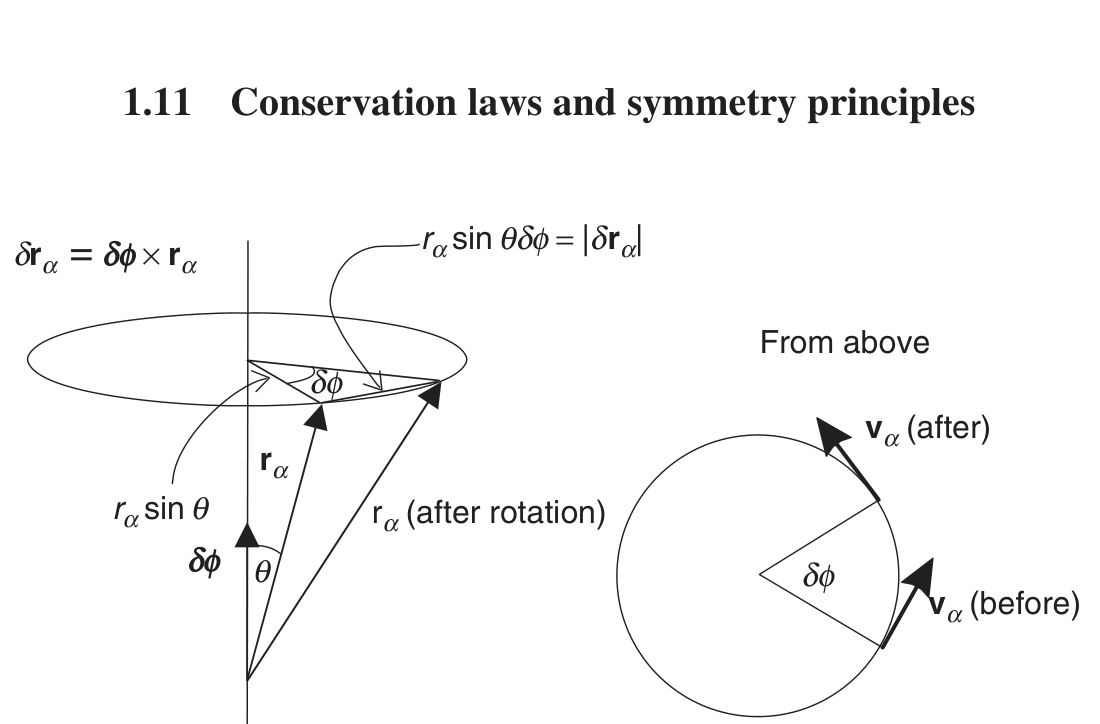
\includegraphics[width=0.55\linewidth]{../Figures/fig_1_10.png}
\caption{图 1.10}
\end{figure}

系统的转动使每个质点的位置改变 $\delta\mathbf{r}_\alpha$，每个质点的速度改变 $\delta\mathbf{v}_\alpha$。

我们现在以更高级的方式处理这个问题，证明角动量守恒是空间各向同性的结果。考虑一个绕某个轴转过虚角度 $\delta\phi$ 的力学系统。设 $\delta\boldsymbol{\phi}$ 是沿转轴方向、大小为 $\delta\phi$ 的矢量。把坐标原点放在转轴上。由于转动，系统中的每个质点都位移某个距离 $\delta\mathbf{r}_\alpha$，如果质点具有速度 $\mathbf{v}_\alpha$，速度矢量的方向将改变 $\delta\mathbf{v}_\alpha$。

如果空间是各向同性的，转动对拉格朗日量没有影响，所以 $\delta L = 0$。即
$$
0 = \delta L = \sum_{\alpha}\left(\frac{\partial L}{\partial \mathbf{r}_\alpha}\cdot\delta\mathbf{r}_\alpha + \frac{\partial L}{\partial \mathbf{v}_\alpha}\cdot\delta\mathbf{v}_\alpha\right).
$$
（注意，在这种情况下，质点的速度不是常数。）

我们再次用拉格朗日方程把 $\frac{\partial L}{\partial \mathbf{r}_\alpha}$ 替换为 $\frac{d}{dt}\frac{\partial L}{\partial \mathbf{v}_\alpha} = \frac{d\mathbf{p}_\alpha}{dt} = \dot{\mathbf{p}}_\alpha$，并写
$$
\sum_{\alpha}\left(\dot{\mathbf{p}}_\alpha\cdot\delta\mathbf{r}_\alpha + \mathbf{p}_\alpha\cdot\delta\mathbf{v}_\alpha\right) = 0.
$$
从图中，$|\delta\mathbf{r}| = r\sin\theta\,\delta\phi$。但由于 $\delta\mathbf{r}$ 同时垂直于 $\mathbf{r}$ 和 $\delta\boldsymbol{\phi}$，我们可以写 $\delta\mathbf{r} = \delta\boldsymbol{\phi}\times\mathbf{r}$。类似地，$\delta\mathbf{v} = \delta\boldsymbol{\phi}\times\mathbf{v}$。因此，
$$
\sum_{\alpha}\left(\dot{\mathbf{p}}_\alpha\cdot(\delta\boldsymbol{\phi}\times\mathbf{r}_\alpha) + \mathbf{p}_\alpha\cdot(\delta\boldsymbol{\phi}\times\mathbf{v}_\alpha)\right) = 0.
$$
交换点乘和叉乘的次序，我们得到
$$
\sum_{\alpha}\delta\boldsymbol{\phi}\cdot\left(\mathbf{r}_\alpha\times\dot{\mathbf{p}}_\alpha + \dot{\mathbf{r}}_\alpha\times\mathbf{p}_\alpha\right) = \delta\boldsymbol{\phi}\cdot\sum_{\alpha}\frac{d}{dt}\left(\mathbf{r}_\alpha\times\mathbf{p}_\alpha\right) = 0.
$$
因此，由于 $\delta\boldsymbol{\phi} \neq 0$，
$$
\sum_{\alpha}\frac{d}{dt}(\mathbf{r}_\alpha\times\mathbf{p}_\alpha) = \frac{d}{dt}\sum_{\alpha}\mathbf{r}_\alpha\times\mathbf{p}_\alpha = \frac{d\mathbf{L}}{dt} = 0,
$$
其中 $\mathbf{L}$ 是总角动量。也就是说，空间各向同性导致角动量守恒。（注意不要把总矢量角动量 $\mathbf{L}$ 与拉格朗日量 $L$ 混淆。）

\begin{exercise}
用初等力学方法证明：如果没有净外力矩作用在系统上，质点系统的角动量就是常数。注意你必须援引强形式的牛顿第三定律。
\end{exercise}

\subsection*{1.11.4  能量守恒与功函数}

考虑单个质点的动能。在初级物理中，我们学过功--能定理，它表明：外力对质点所做的净功，将导致质点动能的等量增加。按定义，功为
$$
W = \int \mathbf{F}\cdot d\mathbf{s}.
$$
因此，受力 $\mathbf{F}$ 作用的质点从点 1 到点 2 的动能增加为
$$
T_2 - T_1 = \int_1^2 \mathbf{F}\cdot d\mathbf{s}.
$$
如果力是保守的，量 $\mathbf{F}\cdot d\mathbf{s}$ 就是一个标量量的微分，这个标量量记为 $U$，称为"功函数"。在现代术语中，功函数的概念已被势能（$V$）所取代，势能定义为功函数的负值：
$$
V = -U.
$$
这意味着，如果力是保守的，它可以用一个标量函数的梯度来表示，于是
$$
\mathbf{F} = -\nabla V.
$$
那么功--能定理给出
$$
T_2 - T_1 = \int_1^2 -\nabla V\cdot d\mathbf{s}.
$$
但 $\nabla V\cdot d\mathbf{s} = dV$，所以
$$
T_2 - T_1 = -(V_2 - V_1),
$$
或
$$
T_2 + V_2 = T_1 + V_1.
$$
这个方程表达机械能守恒；它表明，在保守力作用下，系统从一种位形到另一种位形的过程中，有一个量保持不变。这个量当然就是总机械能 $E = T + V$。

力是保守的条件是：它等于某个标量函数的负梯度。这等价于要求力的旋度为零，即 $\nabla\times\mathbf{F} = 0$。

以上关于能量守恒的讨论相当初等。我们现在从高级的角度考察能量，并证明能量守恒来自时间的均匀性。

一般来说，拉格朗日量 $L = L(q, \dot{q}, t)$ 对时间的导数为
$$
\frac{dL}{dt} = \sum_i\frac{\partial L}{\partial q_i}\frac{dq_i}{dt} + \sum_i\frac{\partial L}{\partial \dot{q}_i}\frac{d\dot{q}_i}{dt} + \frac{\partial L}{\partial t}.
$$
由拉格朗日方程，$\frac{\partial L}{\partial q_i} = \frac{d}{dt}\frac{\partial L}{\partial \dot{q}_i}$，所以
$$
\frac{dL}{dt} = \sum_i\left[\dot{q}_i\frac{d}{dt}\frac{\partial L}{\partial \dot{q}_i} + \frac{\partial L}{\partial \dot{q}_i}\frac{d\dot{q}_i}{dt}\right] + \frac{\partial L}{\partial t}.
$$
但注意
$$
\frac{d}{dt}\sum_i\dot{q}_i\frac{\partial L}{\partial \dot{q}_i} = \sum_i\left(\dot{q}_i\frac{d}{dt}\frac{\partial L}{\partial \dot{q}_i} + \frac{d\dot{q}_i}{dt}\frac{\partial L}{\partial \dot{q}_i}\right),
$$
所以前面方程中的求和可以用 $\frac{d}{dt}\sum_i\dot{q}_i\frac{\partial L}{\partial \dot{q}_i}$ 代替，
$$
\frac{dL}{dt} = \frac{d}{dt}\sum_i\dot{q}_i\frac{\partial L}{\partial \dot{q}_i} + \frac{\partial L}{\partial t},
$$
或
$$
\frac{\partial L}{\partial t} = \frac{d}{dt}\left(L - \sum_i\dot{q}_i\frac{\partial L}{\partial \dot{q}_i}\right).
$$
我们现在引入一个新量，称为能量函数 $h$，定义为
$$
h = h(q, \dot{q}, t) = \sum_i\dot{q}_i\frac{\partial L}{\partial \dot{q}_i} - L,
$$
所以
$$
\frac{\partial L}{\partial t} = -\frac{dh}{dt}.
$$
注意 $h$ 依赖于广义位置和广义速度。

让我们假定时间均匀性，使得时间不显式出现在拉格朗日量中。于是 $\frac{\partial L}{\partial t} = 0$，从而
$$
\frac{d}{dt}\left(L - \sum_i\dot{q}_i\frac{\partial L}{\partial \dot{q}_i}\right) = -\frac{dh}{dt} = 0.
$$
也就是说，能量函数是常数。但这是否意味着能量（$E = T + V$）是常数？为了回答这个问题，我们注意到动能具有一般形式
$$
T = T_0 + T_1 + T_2,
$$
其中 $T_0$ 不依赖于速度，$T_1$ 是速度的一次齐次函数，$T_2$ 是速度的二次齐次函数。\footnote{这可以从笛卡尔坐标中的动能出发，利用变换方程 $\xi = \xi(q_1, q_2, \ldots, q_n, t)$ 以及 $\dot{x}_i = \sum_j\frac{\partial \xi}{\partial q_j}\dot{q}_j + \frac{\partial \xi}{\partial t}$ 来证明。参见章末习题 1.12。}（在笛卡尔坐标中，$T_0$ 和 $T_1$ 都为零，$T_2$ 不仅对速度是二次的，而且实际上是速度的二次型，即它包含 $\dot{x}^2$ 而不包含 $\dot{x}\dot{y}$。）

回忆函数 $f(x_1, \ldots, x_n)$ 若满足
$$
f(\alpha x_1, \alpha x_2, \ldots, \alpha x_n) = \alpha^k f(x_1, \ldots, x_n),
$$
则称为 $k$ 次齐次函数。欧拉关于齐次函数的定理指出，若 $f$ 是 $k$ 次齐次的，则
$$
\sum_i x_i\frac{\partial f}{\partial x_i} = kf.
$$
由于动能具有 $T_0 + T_1 + T_2$ 的一般形式，拉格朗日量也具有这种形式：$L = L_0 + L_1 + L_2$。于是由欧拉定理，
$$
\sum_i\dot{q}_i\frac{\partial L_0}{\partial \dot{q}_i} = 0,
$$
$$
\sum_i\dot{q}_i\frac{\partial L_1}{\partial \dot{q}_i} = L_1,
$$
$$
\sum_i\dot{q}_i\frac{\partial L_2}{\partial \dot{q}_i} = 2L_2.
$$
因此，
$$
\sum_i\dot{q}_i\frac{\partial L}{\partial \dot{q}_i} = \sum_i\dot{q}_i\frac{\partial (L_0 + L_1 + L_2)}{\partial \dot{q}_i} = L_1 + 2L_2,
$$
以及
$$
\sum_i\dot{q}_i\frac{\partial L}{\partial \dot{q}_i} - L = (L_1 + 2L_2) - (L_0 + L_1 + L_2) = L_2 - L_0.
$$
如果变换方程不显含 $t$，则 $T = T_2$，即 $T$ 是速度的二次齐次函数。如果 $V$ 不依赖于速度，则 $L_0 = -V$。于是
$$
h = T + V = E.
$$
只要这些条件得到满足，能量函数就等于总能量，总能量就守恒。

如果我们把 $\frac{\partial L}{\partial \dot{q}_i}$ 替换为 $p_i$，能量函数就变换为哈密顿量，它是广义坐标和广义动量的函数：
$$
H = H(q, p, t) = \sum_i\dot{q}_ip_i - L.
$$
能量函数和哈密顿量本质上是一回事，但它们是用不同的变量表示的，即 $h = h(q, \dot{q}, t)$ 和 $H = H(q, p, t)$。（$h$ 依赖于速度，而 $H$ 依赖于动量。）

\begin{exercise}
（a）证明 $\mathbf{F} = -y\hat{\mathbf{i}} + x\hat{\mathbf{j}}$ 不是保守的。（b）证明 $\mathbf{F} = y\hat{\mathbf{i}} + x\hat{\mathbf{j}}$ 是保守的。
\end{exercise}

\begin{exercise}
证明 $\mathbf{F} = 3x^2y\hat{\mathbf{i}} + (x^3 + 1)\hat{\mathbf{j}} + 9z^2\hat{\mathbf{k}}$ 是保守的。
\end{exercise}

\begin{exercise}
证明保守力的旋度为零。
\end{exercise}

\begin{exercise}
证明欧拉定理。（提示：对 $f(tx, ty, tz) = t^k f(x, y, z)$ 关于 $t$ 求导，然后令 $t = 1$。）
\end{exercise}

\begin{exercise}
证明 $z^2\ln(x/y)$ 是二次齐次的。
\end{exercise}

\begin{exercise}
证明
$$
\sum_i\dot{q}_i\frac{\partial L_2}{\partial \dot{q}_i} = 2L_2.
$$
\end{exercise}

\subsection*{位力定理}

位力定理指出：对有界的保守系统（如绕恒星运行的行星），动能的平均值与势能的平均值成正比。（对行星/恒星系统，我们发现 $\langle T\rangle = -\frac{1}{2}\langle V\rangle$。）我们现在来证明这个定理。

在笛卡尔坐标中，动能是只依赖于速度的齐次二次函数，所以欧拉定理给出
$$
\sum_{\alpha}\mathbf{v}_\alpha\cdot\frac{\partial T}{\partial \mathbf{v}_\alpha} = 2T.
$$
只要势能不依赖于速度，动量就可以表示为
$$
\mathbf{p}_\alpha = \frac{\partial T}{\partial \mathbf{v}_\alpha},
$$
从而
$$
2T = \sum_{\alpha}\mathbf{p}_\alpha\cdot\mathbf{v}_\alpha = \sum_{\alpha}\mathbf{p}_\alpha\cdot\frac{d\mathbf{r}_\alpha}{dt}.
$$
但
$$
\frac{d}{dt}\sum_{\alpha}\mathbf{p}_\alpha\cdot\mathbf{r}_\alpha = \sum_{\alpha}\mathbf{p}_\alpha\cdot\frac{d\mathbf{r}_\alpha}{dt} + \sum_{\alpha}\frac{d\mathbf{p}_\alpha}{dt}\cdot\mathbf{r}_\alpha.
$$
因此
$$
2T = \frac{d}{dt}\sum_{\alpha}\mathbf{p}_\alpha\cdot\mathbf{r}_\alpha - \sum_{\alpha}\frac{d\mathbf{p}_\alpha}{dt}\cdot\mathbf{r}_\alpha.
$$
现在由牛顿第二定律，对保守系统，
$$
\frac{d\mathbf{p}_\alpha}{dt} = \mathbf{F}_\alpha = -\frac{\partial V}{\partial \mathbf{r}_\alpha},
$$
所以
$$
2T = \frac{d}{dt}\sum_{\alpha}\mathbf{p}_\alpha\cdot\mathbf{r}_\alpha + \sum_{\alpha}\frac{\partial V}{\partial \mathbf{r}_\alpha}\cdot\mathbf{r}_\alpha.
$$
让我们求这个方程中所有项的平均值：
$$
\langle 2T\rangle = \left\langle\frac{d}{dt}\sum_{\alpha}\mathbf{p}_\alpha\cdot\mathbf{r}_\alpha\right\rangle + \left\langle\sum_{\alpha}\mathbf{r}_\alpha\cdot\frac{\partial V}{\partial \mathbf{r}_\alpha}\right\rangle.
$$
回忆函数 $f(t)$ 的时间平均为
$$
\langle f(t)\rangle = \lim_{\tau\to\infty}\frac{1}{\tau}\int_0^{\tau} f(t)\,dt,
$$
所以
$$
\left\langle\frac{d}{dt}\sum_{\alpha}\mathbf{p}_\alpha\cdot\mathbf{r}_\alpha\right\rangle = \lim_{\tau\to\infty}\frac{1}{\tau}\int_0^{\tau}\frac{d}{dt}\left(\sum_{\alpha}\mathbf{p}_\alpha\cdot\mathbf{r}_\alpha\right)dt = \lim_{\tau\to\infty}\frac{\sum_{\alpha}\mathbf{p}_\alpha\cdot\mathbf{r}_\alpha(\tau) - \sum_{\alpha}\mathbf{p}_\alpha\cdot\mathbf{r}_\alpha(0)}{\tau} = 0,
$$
其中我们假定 $\sum_{\alpha}\mathbf{p}_\alpha\cdot\mathbf{r}_\alpha$ 在所有时刻都保持有限。换句话说，我们假定运动是有界的，所以分子有限而分母趋于无穷大。

我们剩下
$$
2\langle T\rangle = \left\langle\sum_{\alpha}\mathbf{r}_\alpha\cdot\frac{\partial V}{\partial \mathbf{r}_\alpha}\right\rangle.
$$
如果势能是位置的 $k$ 次齐次函数，那么由欧拉定理，右边为 $kV$，于是
$$
2\langle T\rangle = k\langle V\rangle.
$$
因此，例如，对引力场中质量为 $m$ 的质点，
$$
V = -\frac{GMm}{r},
$$
所以 $k = -1$，且
$$
2\langle T\rangle = -\langle V\rangle.
$$
由于 $E = T + V$，我们看到 $\langle E\rangle = -\langle T\rangle$，这表明总能量为负，且平均动能的量值是平均势能量值的一半。

再举一个例子，考虑弹簧上的质量。势能为 $V = \frac{1}{2}Kx^2$，所以 $k = 2$，且 $2\langle T\rangle = 2\langle V\rangle$，即 $\langle T\rangle = \langle V\rangle$。

\section*{1.12  习题}

\subsection*{习题 1.1}
有一个故事，讲的是一个物理学家因闯红灯而吃了罚单。作为一位聪明人，这位物理学家向法官证明：要么无法停车，要么无法继续前行，而不闯红灯或超速。在这个问题中，我们来确定这个故事是可信的，还是某个过度劳累的研究生凭空想象的。假设这位物理学家以恒定速度 $v_0$（等于限速）开车。当交通灯由绿变黄时，汽车距交叉路口距离为 $d$。物理学家有反应时间 $\tau$，汽车以恒定减速度 $a_c$ 制动。黄灯持续时间为 $t_y$。确定使汽车既不能停下、也不能以 $v_0$ 继续前行而不闯红灯的条件。另外，用 $\tau$、$t_y$、$a_c$ 和 $v_0$ 的实际数值确定这种情况是否真的会发生。（用简单的运动学关系求解。）

\subsection*{习题 1.2}
质量为 $M$、半径为 $R$ 的圆柱体竖立在桌子上，距桌边距离为 $L$。一根绳子绕在圆柱上。绳子的自由端绕过无摩擦的滑轮，从桌边垂下。绳子自由端挂一质量为 $m$ 的重物。求线轴到达桌边所需的时间。
\begin{figure}[h]
\centering
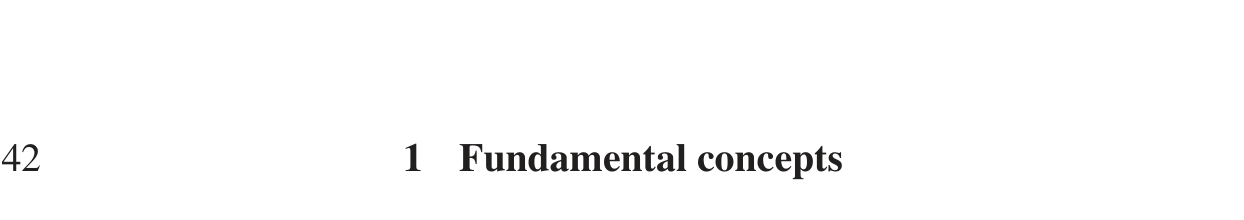
\includegraphics[width=0.55\linewidth]{../Figures/fig_1_11.png}
\caption{图 1.11}
\end{figure}

无摩擦桌面上的圆柱体。

\subsection*{习题 1.3}
一根绳子跨过一只无质量的滑轮。绳子的两端各绕在一个竖直圆环上。两个圆环都可以下降（绳子随圆环下降而解开），但如果一个圆环比另一个重得多，它就能使较轻的圆环上升。圆环的质量为 $M_1$ 和 $M_2$，半径为 $R_1$ 和 $R_2$。证明绳中的张力为 $\tau = gM_1M_2(M_1 + M_2)^{-1}$。
\begin{figure}[h]
\centering
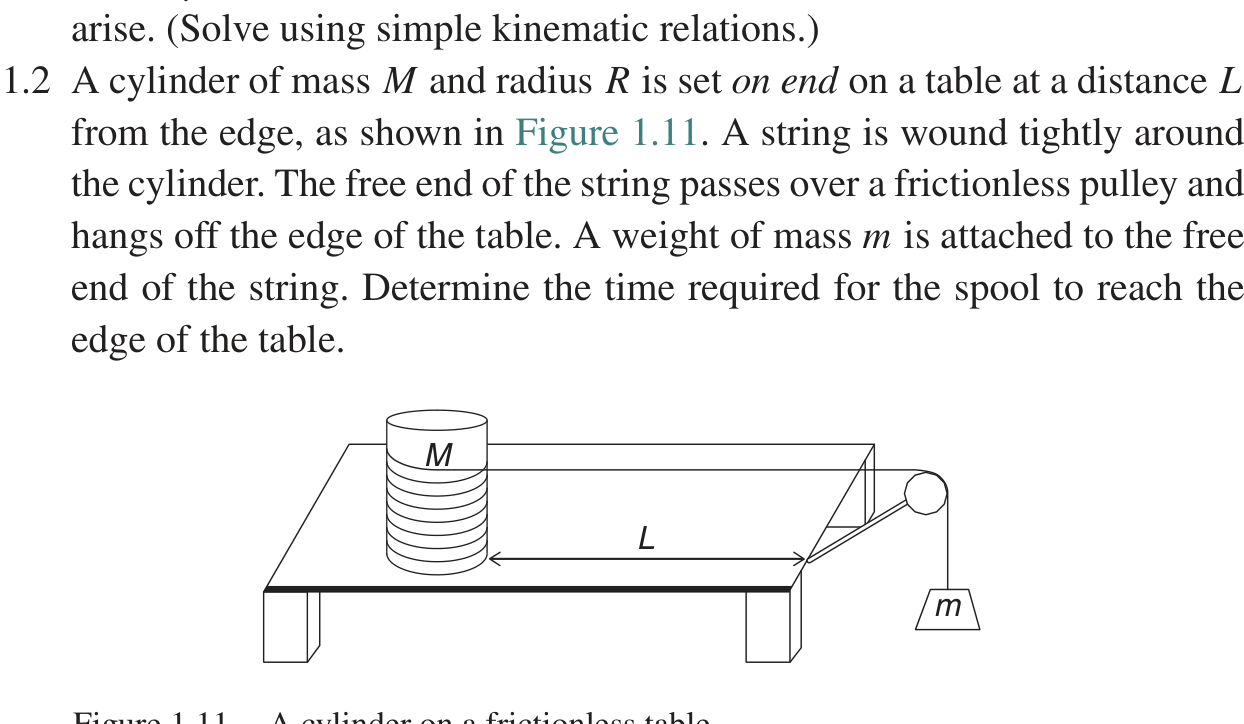
\includegraphics[width=0.55\linewidth]{../Figures/fig_1_12.png}
\caption{图 1.12}
\end{figure}

两个圆环挂在滑轮上。随着圆环下降，绳子解开。

\subsection*{习题 1.4}
双极坐标 $\eta$ 和 $\zeta$ 的变换方程为
$$
x = \frac{a\sinh\eta}{\cosh\eta - \cos\zeta}, \qquad y = \frac{a\sin\zeta}{\cosh\eta - \cos\zeta}.
$$
（a）证明逆变换存在。（b）用 $x$ 和 $y$ 求 $\eta$ 和 $\zeta$ 的表达式。

\subsection*{习题 1.5}
质量为 $m$、半径为 $a$ 的圆盘在倾角为 $\alpha$ 的完全粗糙斜面上滚下。确定运动方程和作用于圆盘上的约束。

\subsection*{习题 1.6}
长度为 $l$、质量为 $m$ 的摆安装在质量为 $M$ 的小车上，小车可以自由地沿轨道滚动。没有摩擦。写出摆/小车系统的拉格朗日量。

\subsection*{习题 1.7}
从定义
$$
T = \frac{1}{2}\sum_{i=1}^{N}m_i\left(\dot{x}_i^2 + \dot{y}_i^2 + \dot{z}_i^2\right)
$$
和变换方程出发，证明
$$
T = \sum_{j=1}^{3N}\sum_{k=1}^{3N}\frac{1}{2}A_{jk}\dot{q}_j\dot{q}_k + \sum_{j=1}^{3N}B_j\dot{q}_j + T_0,
$$
其中
$$
A_{jk} = \sum_{i=1}^{N}m_i\left(\frac{\partial \xi_i}{\partial q_j}\frac{\partial \xi_i}{\partial q_k} + \frac{\partial y_i}{\partial q_j}\frac{\partial y_i}{\partial q_k} + \frac{\partial z_i}{\partial q_j}\frac{\partial z_i}{\partial q_k}\right),
$$
$$
B_j = \sum_{i=1}^{N}m_i\left(\frac{\partial \xi_i}{\partial q_j}\frac{\partial \xi_i}{\partial t} + \frac{\partial y_i}{\partial q_j}\frac{\partial y_i}{\partial t} + \frac{\partial z_i}{\partial q_j}\frac{\partial z_i}{\partial t}\right),
$$
$$
T_0 = \frac{1}{2}\sum_{i=1}^{N}m_i\left[\left(\frac{\partial \xi_i}{\partial t}\right)^2 + \left(\frac{\partial y_i}{\partial t}\right)^2 + \left(\frac{\partial z_i}{\partial t}\right)^2\right].
$$
